\documentclass[report.tex]{subfiles}

% \usepackage[section]{placeins}

\begin{document}

\pagebreak
\chapter[Chương 3. Triển khai ứng dụng]{Triển khai ứng dụng}
% \addcontentsline{toc}{chapter}{\textbf{Chương 3. Triển khai ứng dụng}}

\section{Môi trường phát triển}

\begin{itemize}
\item IDE: Visual Studio Code, Jetbrains Intellij
\item Java SDK 11
\item Build và Dependency Management: Maven
\item Trình duyệt Google Chrome hoặc Firefox
\item Docker
\end{itemize}

\section{Các bước triển khai hệ thống}

\begin{itemize}
\item Khởi tạo database trên PostgreSQL
\item Khởi tạo service Eureka
\item Khởi tạo các service

\end{itemize}

\textbf{Triển khai hệ thống giám sát:}

\begin{itemize}
\item Cấu hình endpoint `/actuator/prometheus` ở từng service để Prometheus thu thập số liệu
\item Cấu hình địa chỉ các service cho Prometheus:

\begin{minted}{yaml}
scrape_configs:
  - job_name: 'prometheus-api-scraper'
    metrics_path: '/actuator/prometheus'
    static_configs:
      - targets: [ '<service-host>:5000' ]
        labels:
          application: 'api-gateway'
      - targets: [ '<service-host>:5001' ]
        labels:
          application: 'user-service'
      - targets: [ '<service-host>:5002' ]
        labels:
          application: 'syllabus-service'
      - targets: [ '<service-host>:5003' ]
        labels:
          application: 'program-service'
      - targets: [ '<service-host>:5004' ]
        labels:
          application: 'class-service'
      - targets: [ '<service-host>:5005' ]
        labels:
          application: 'auth-service'
\end{minted}
\item Cấu hình datasource cho Grafana để trỏ tới Prometheus
\begin{minted}{yaml}
datasources:
  - name: Prometheus
    type: prometheus
    url: http://<service-host>:39090
\end{minted}
\item Khởi tạo Zipkin để trace request
\end{itemize}

\begin{figure}[!htb]
{\centering
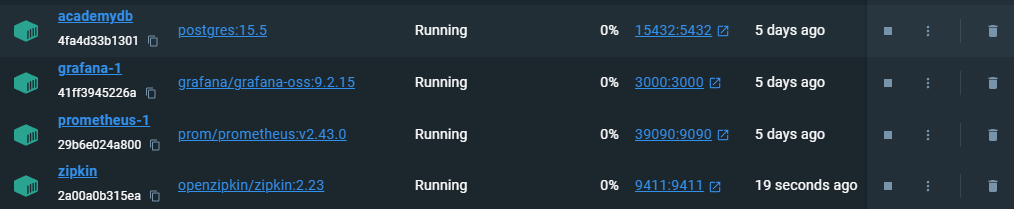
\includegraphics[width=380px]{../meta/ui.docker-compose.png}
\caption{Các service được triển khai trên Docker}
\par
}
\end{figure}
\FloatBarrier

\section{Giao diện người dùng}

\subsection{Đăng nhập}

\begin{figure}[!htb]
{\centering
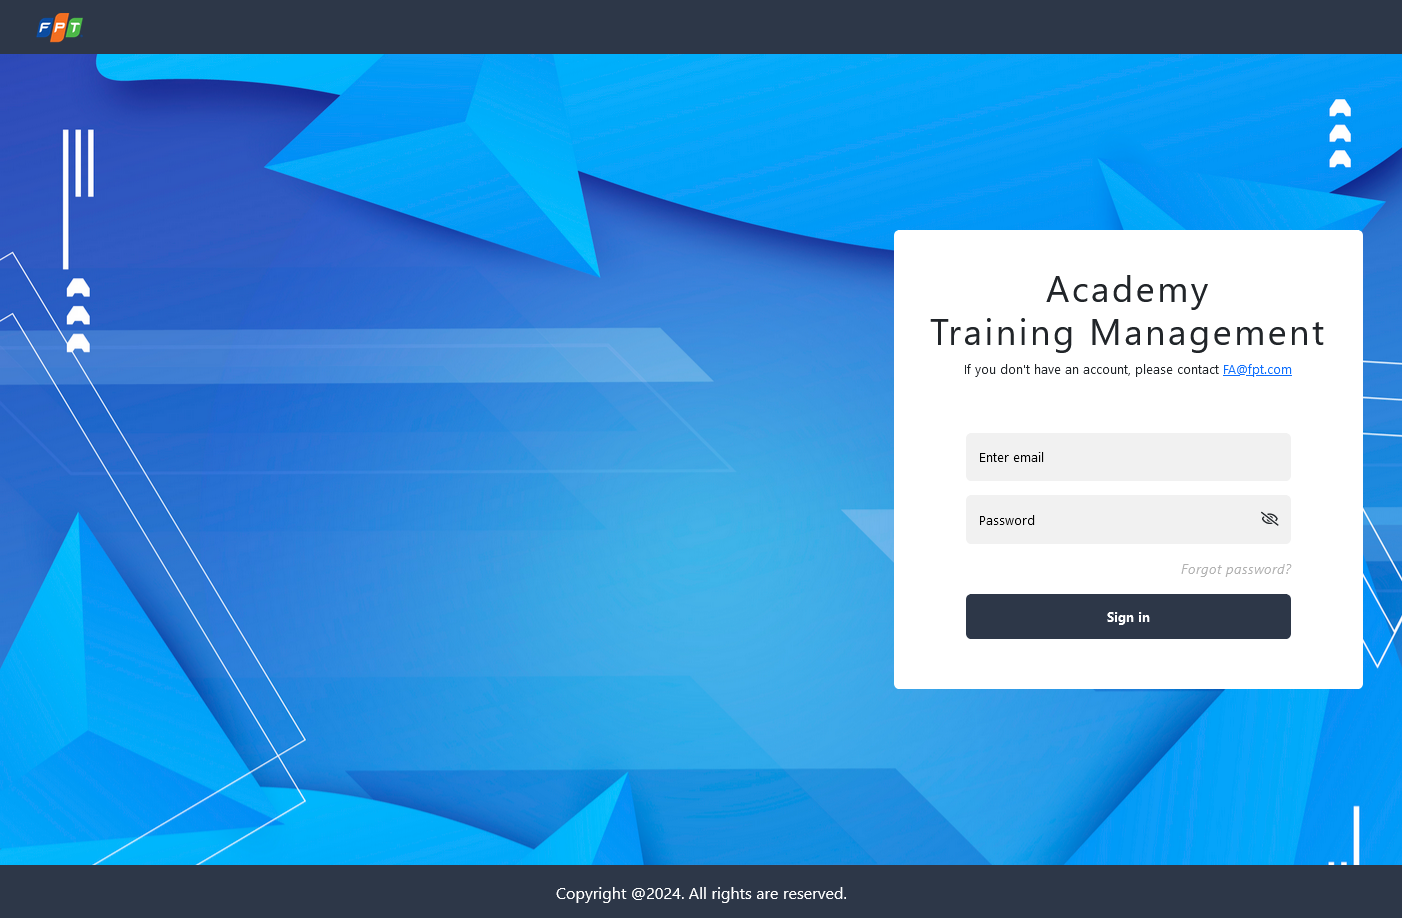
\includegraphics[width=380px]{../meta/ui.login.png}
\caption{Màn hình Đăng nhập}
\par
}
\end{figure}
\FloatBarrier

Màn hình để người dùng đăng nhập mỗi khi muốn sử dụng hệ thống để
xem những thông tin về lớp học cũng như thông tin cá nhân trong hệ thống.

\subsection{Thông tin người dùng}

\begin{figure}[!htb]
{\centering
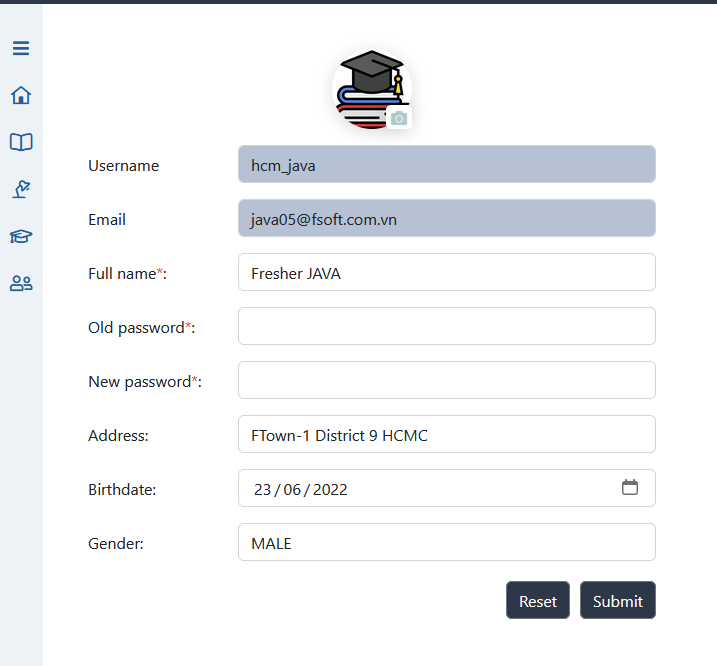
\includegraphics[width=380px]{../meta/ui.user-info.png}
\caption{Màn hình Xem/chỉnh sửa thông tin người dùng}
\par
}
\end{figure}
\FloatBarrier

Người dùng có thể thay đổi mật khẩu hay thông tin cá nhân khi cần thiết,
đối với tên đăng nhập username và email không được thay đổi.

\subsection{Người dùng}

\begin{figure}[!htb]
{\centering
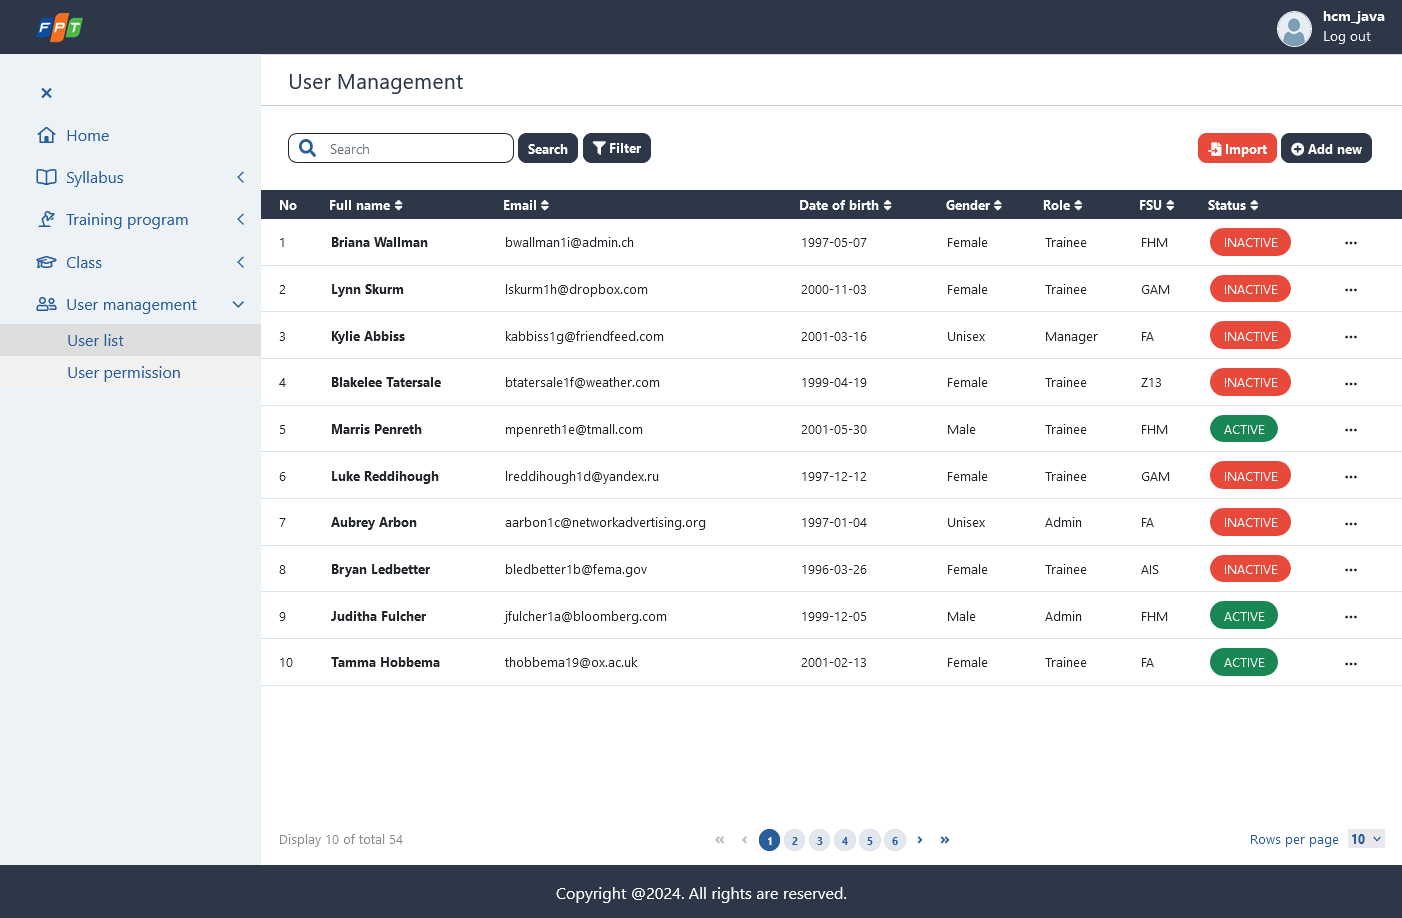
\includegraphics[width=380px]{../meta/ui.user-list.png}
\caption{Màn hình Quản lí danh sách người dùng}
\par
}
\end{figure}
\FloatBarrier

\begin{figure}[!htb]
{\centering
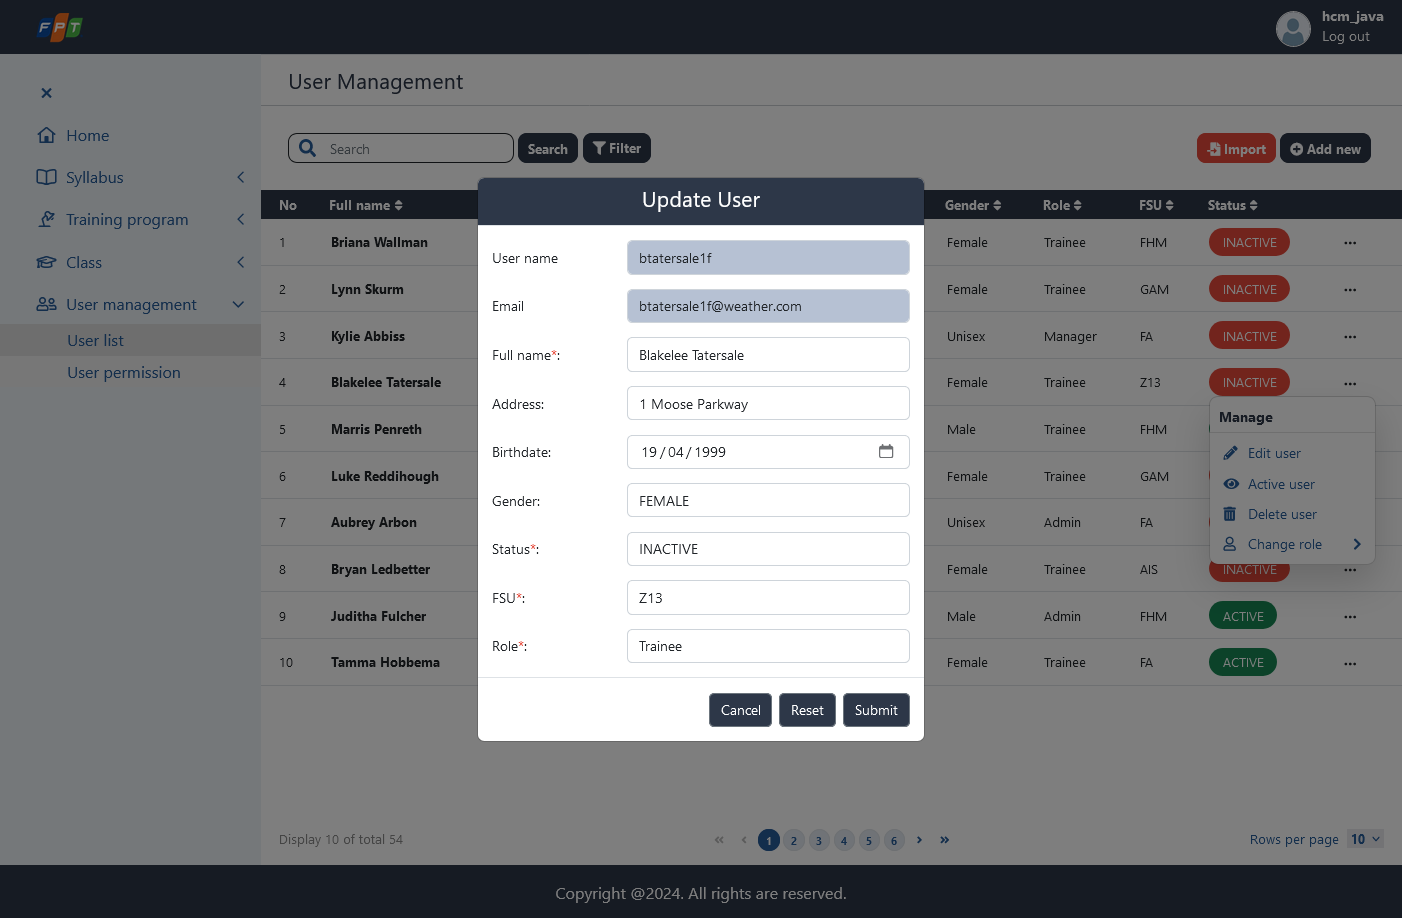
\includegraphics[width=380px]{../meta/ui.user-admin-update.png}
\caption{Màn hình tạo/chỉnh sửa thông tin người dùng}
\par
}
\end{figure}
\FloatBarrier

Người quản trị có thể xem và thay đổi thông tin người dùng khi cần thiết,
đối với tên đăng nhập không được thay đổi.

\subsection{Nội dung đào tạo}

Các giao diện chức năng cho phép xem thông tin, xóa, sửa, phân trang, lọc/tìm kiếm
NDDT.

\begin{figure}[!htb]
{\centering
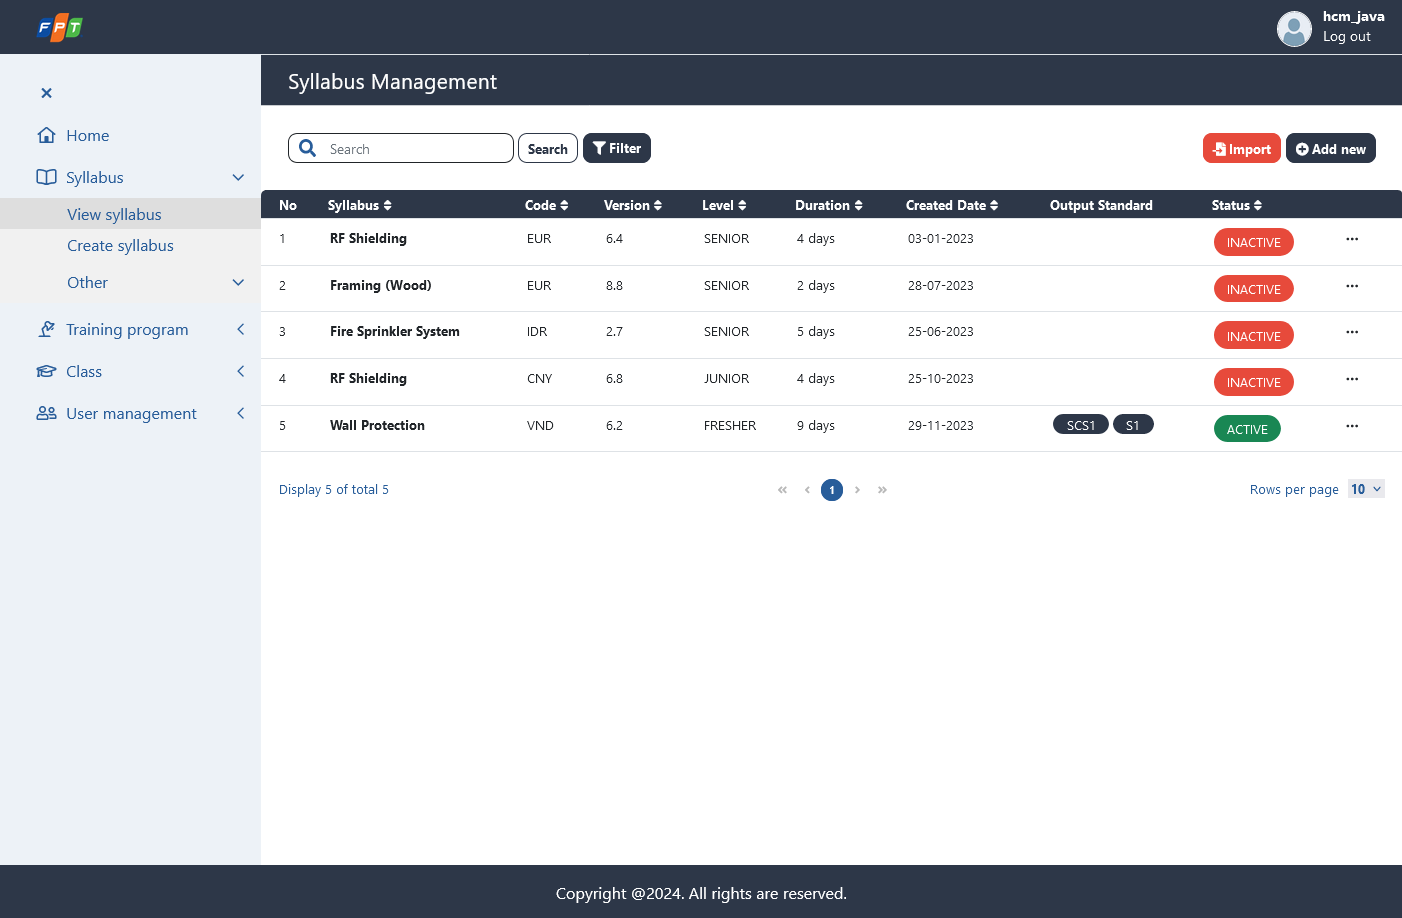
\includegraphics[width=380px]{../meta/ui.syllabus-list.png}
\caption{Màn hình Danh sách nội dung đào tạo}
\par
}
\end{figure}
\FloatBarrier

{\centering
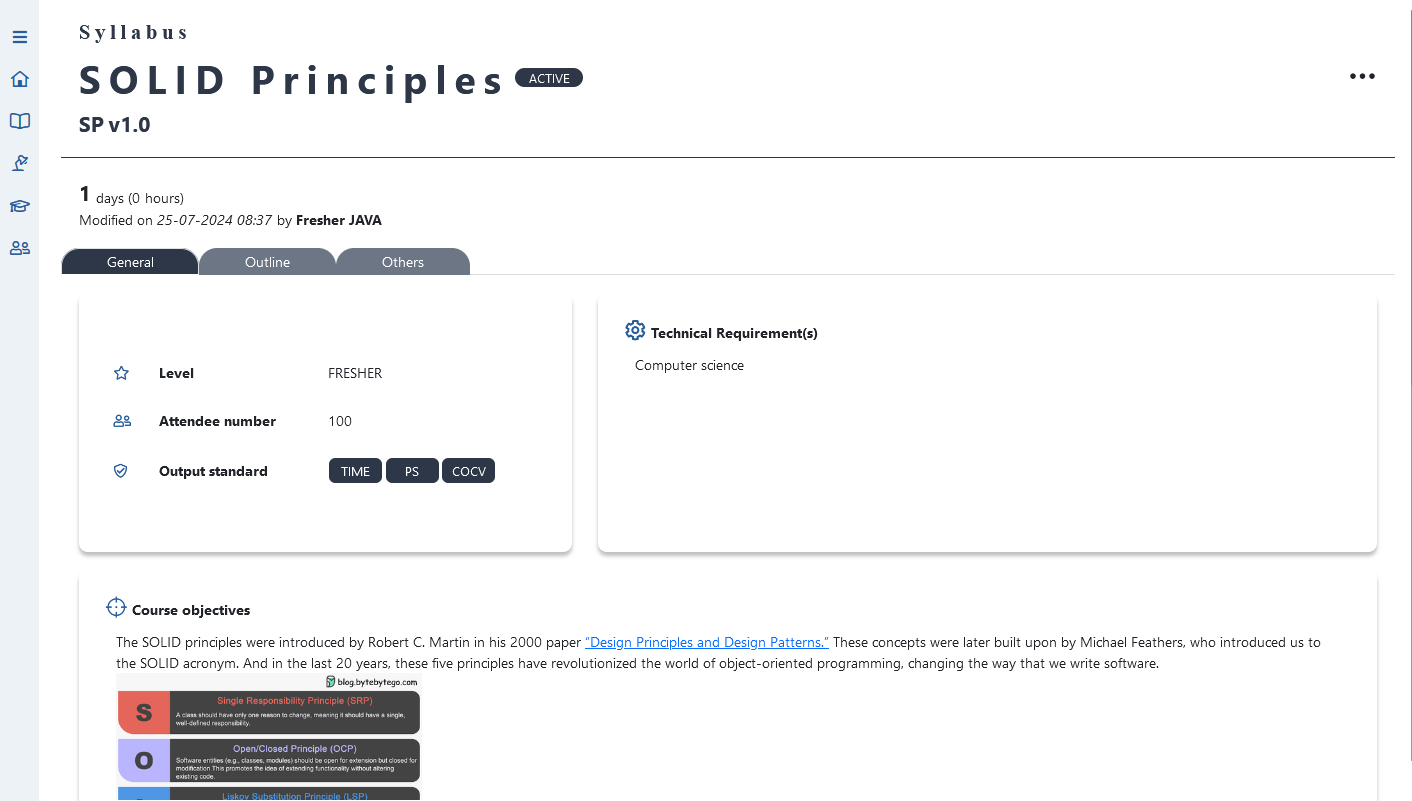
\includegraphics[width=380px]{../meta/ui.syllabus-detail-1.png}
\par
}
{\centering
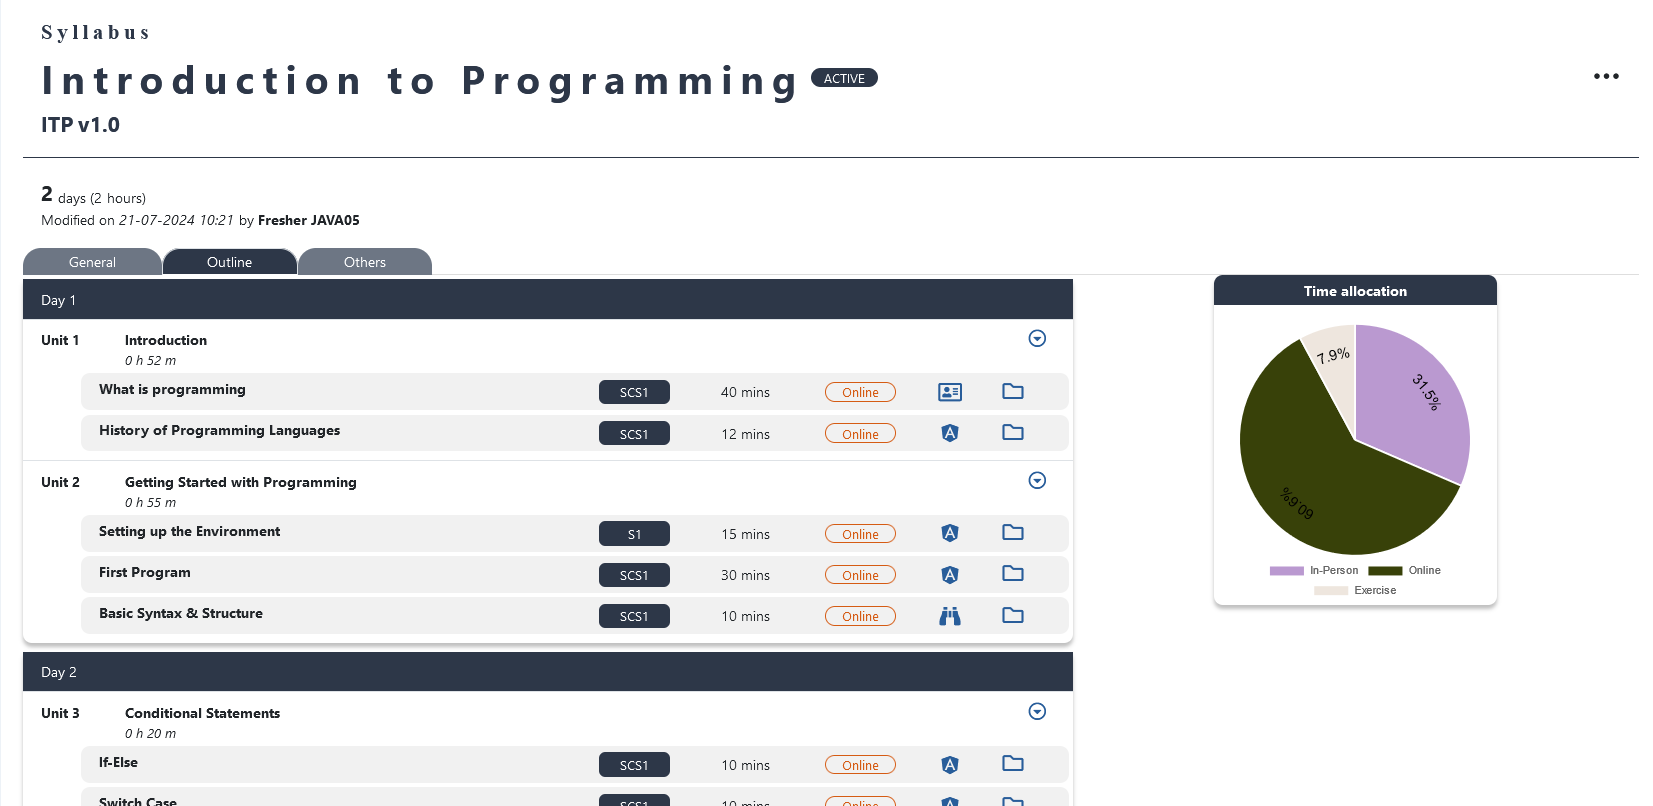
\includegraphics[width=380px]{../meta/ui.syllabus-detail-2.png}
\par
}
\begin{figure}[!htb]
{\centering
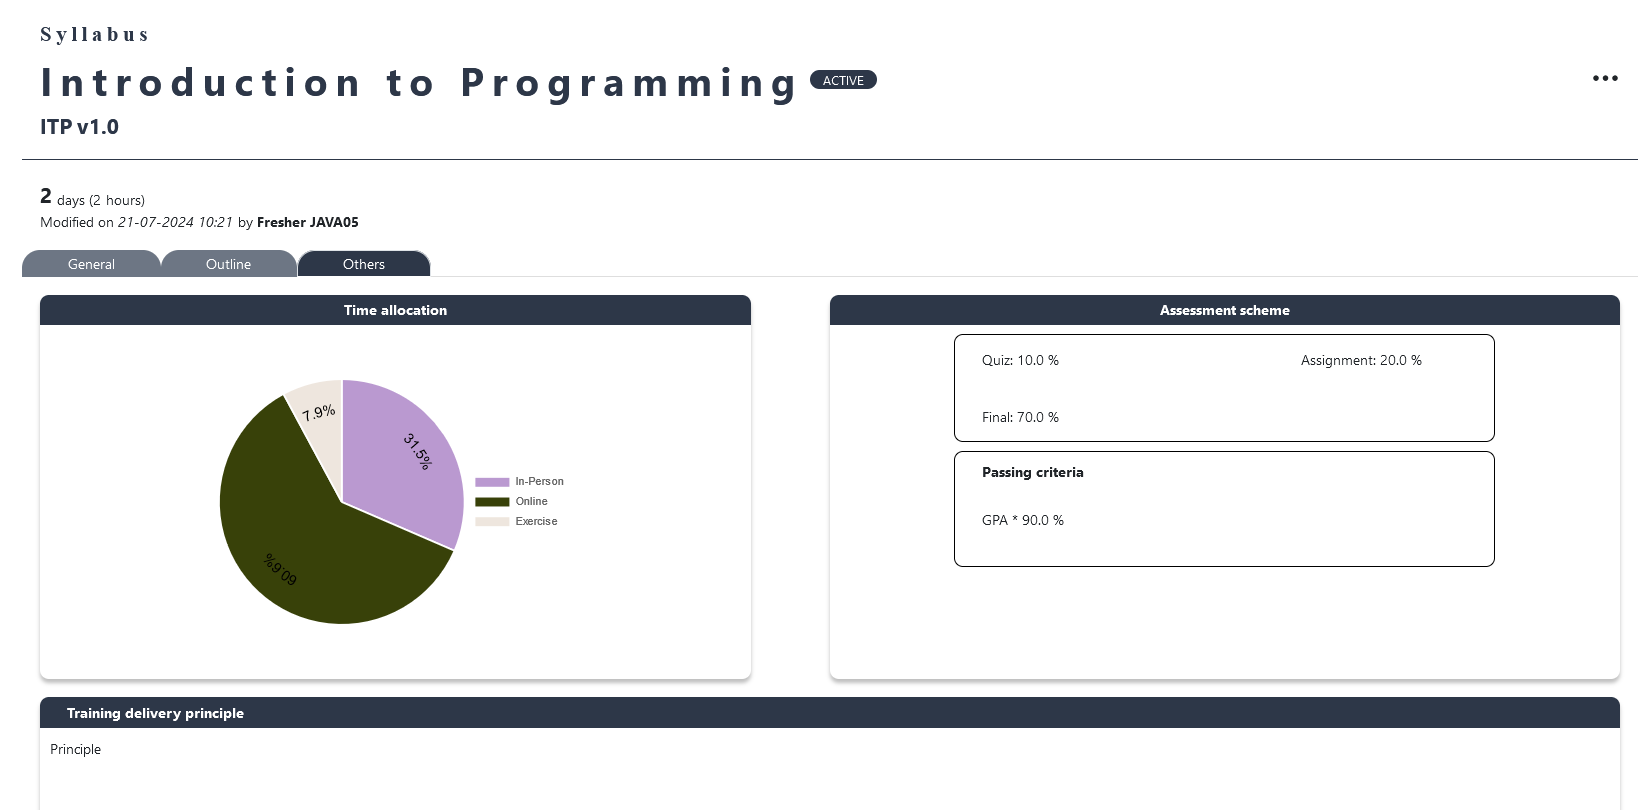
\includegraphics[width=380px]{../meta/ui.syllabus-detail-3.png}
\caption{Màn hình Thông tin nội dung đào tạo}
\par
}
\end{figure}
\FloatBarrier

\subsection{Tài liệu đào tạo}

Giao diện hiển thị các tài liệu mà quản trị viên đã thêm vào mỗi chương đào tạo.
Ở đây, người dùng có thể xem, sửa, xóa các tài liệu ra khỏi NDDT.

\begin{figure}[!htb]
{\centering
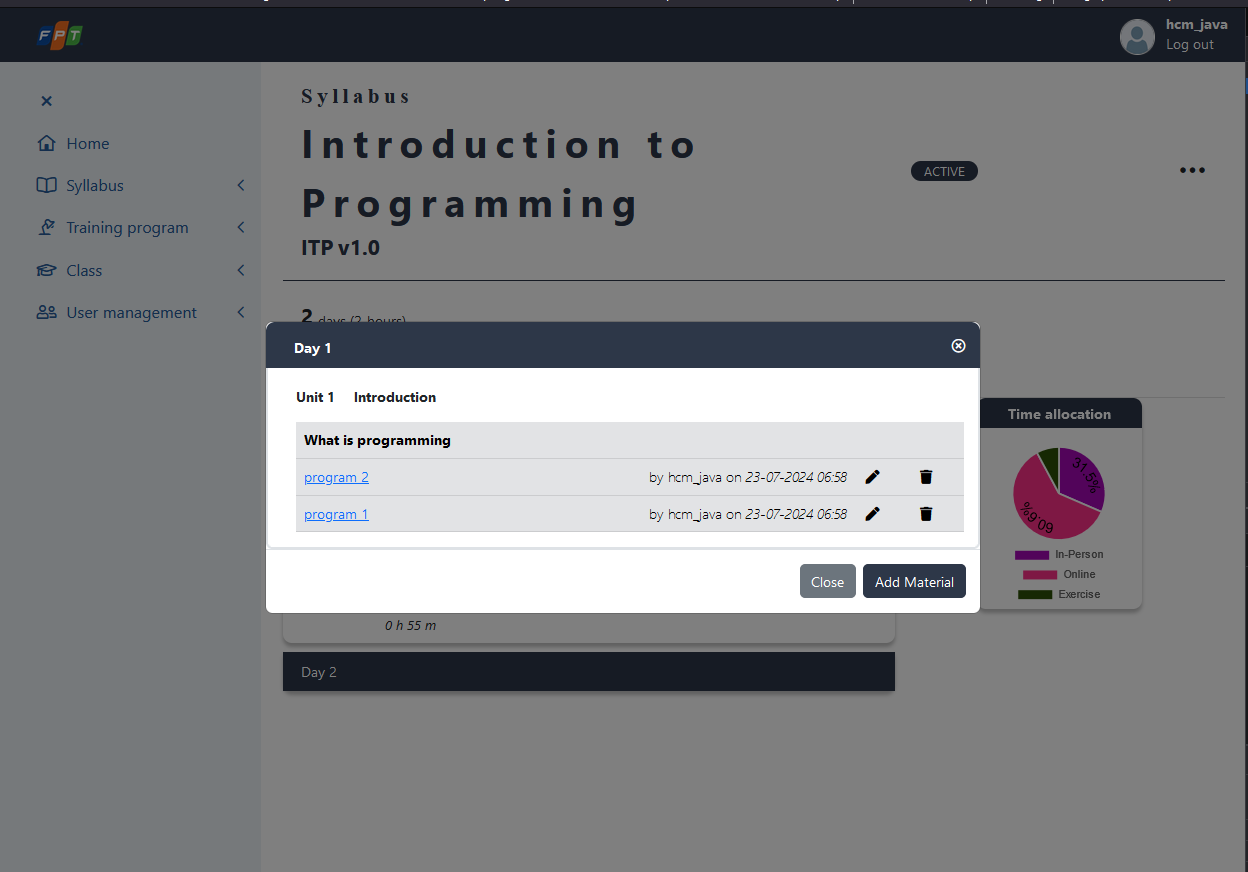
\includegraphics[width=380px]{../meta/ui.material-list.png}
\caption{Màn hình danh sách tài liệu}
\par
}
\end{figure}
\FloatBarrier

\begin{figure}[!htb]
{\centering
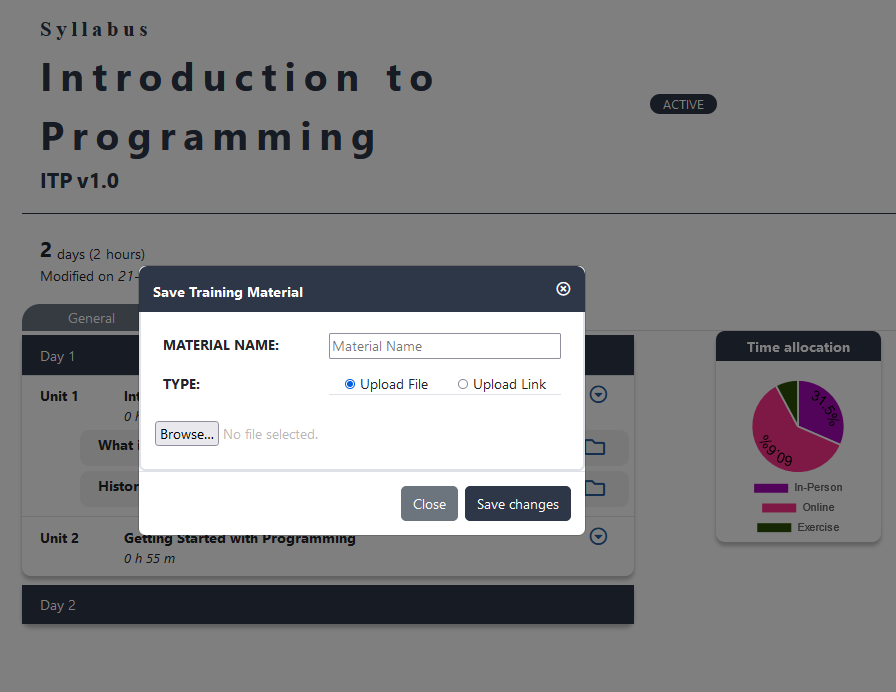
\includegraphics[width=380px]{../meta/ui.material-create1.png}
\caption{Màn hình tạo tài liệu}
\par
}
\end{figure}
\FloatBarrier

\subsection{Chương trình học}

Giao diện chức năng cho phép xem thông tin, xóa, sửa, phân trang, lọc/tìm kiếm chương trình đào tạo.

\begin{figure}[!htb]
{\centering
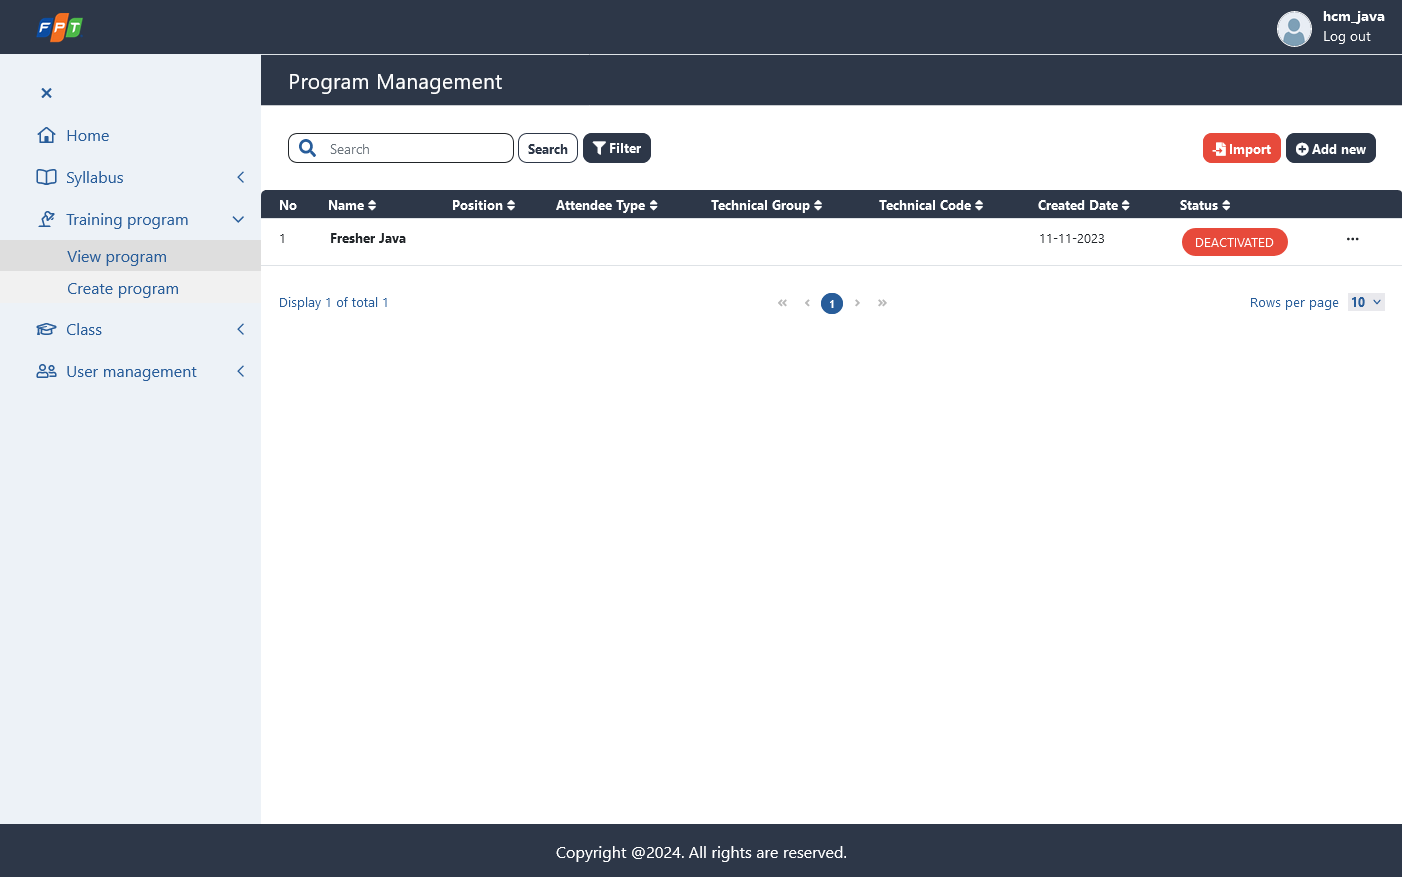
\includegraphics[width=380px]{../meta/ui.program-list.png}
\caption{Màn hình danh sách chương trình học}
\par
}
\end{figure}
\FloatBarrier

\begin{figure}[!htb]
{\centering
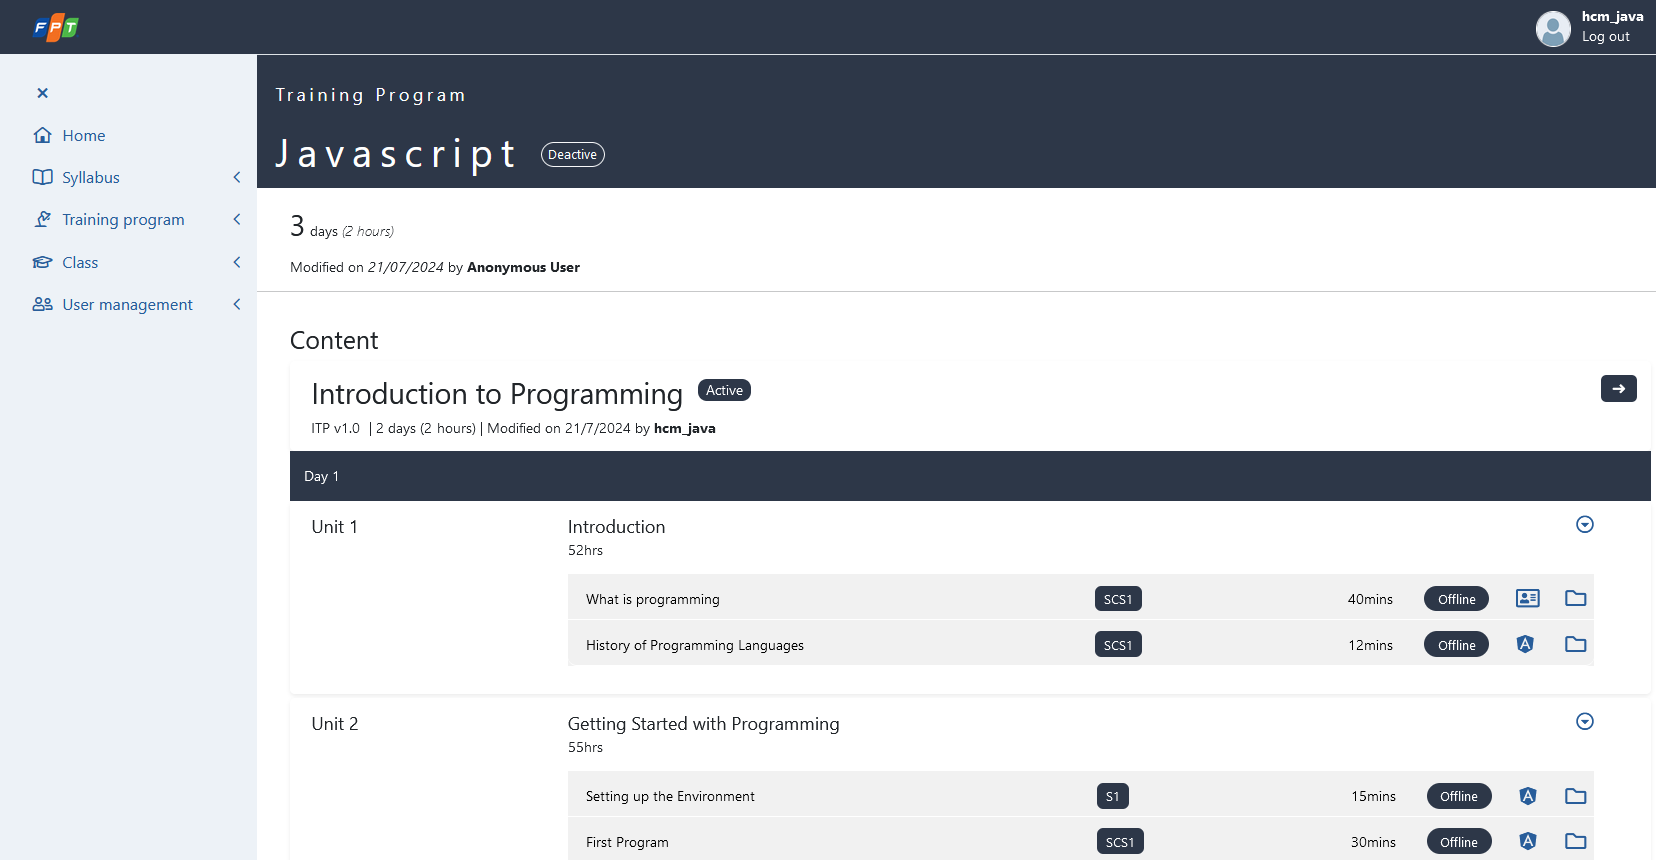
\includegraphics[width=380px]{../meta/ui.program-detail.png}
\caption[Màn hình thông tin CTDT]{Màn hình thông tin tất cả các TLDT bên trong CTDT}
\par
}
\end{figure}
\FloatBarrier

{\centering
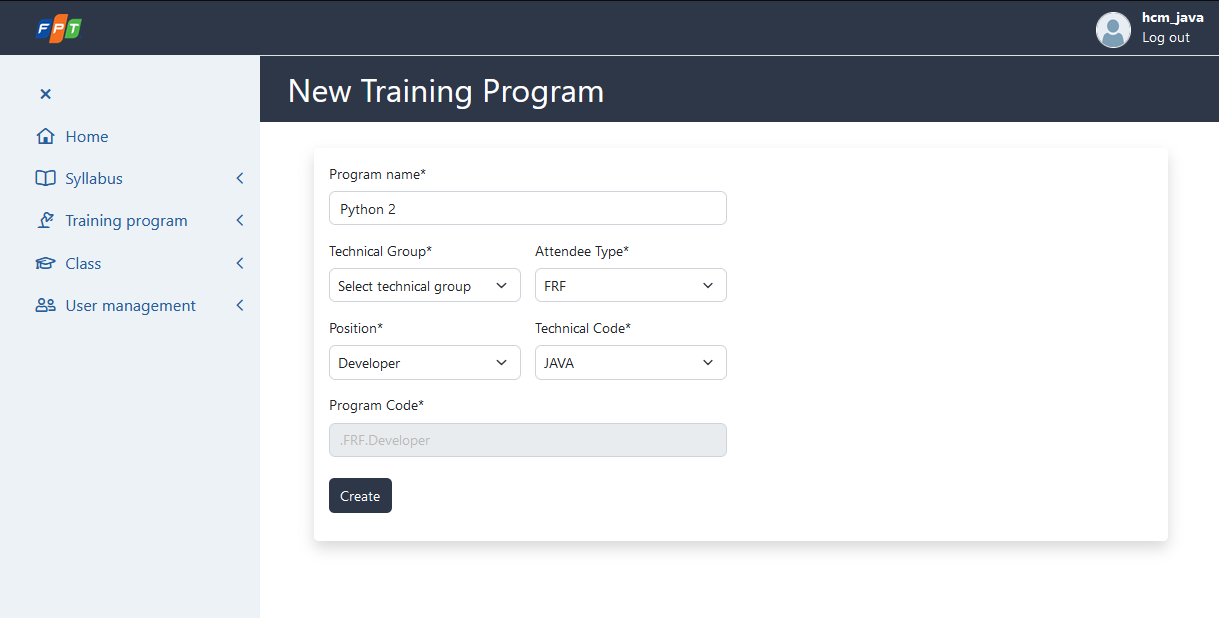
\includegraphics[width=380px]{../meta/ui.program-create-1.png}
\par
}
\begin{figure}[!htb]
{\centering
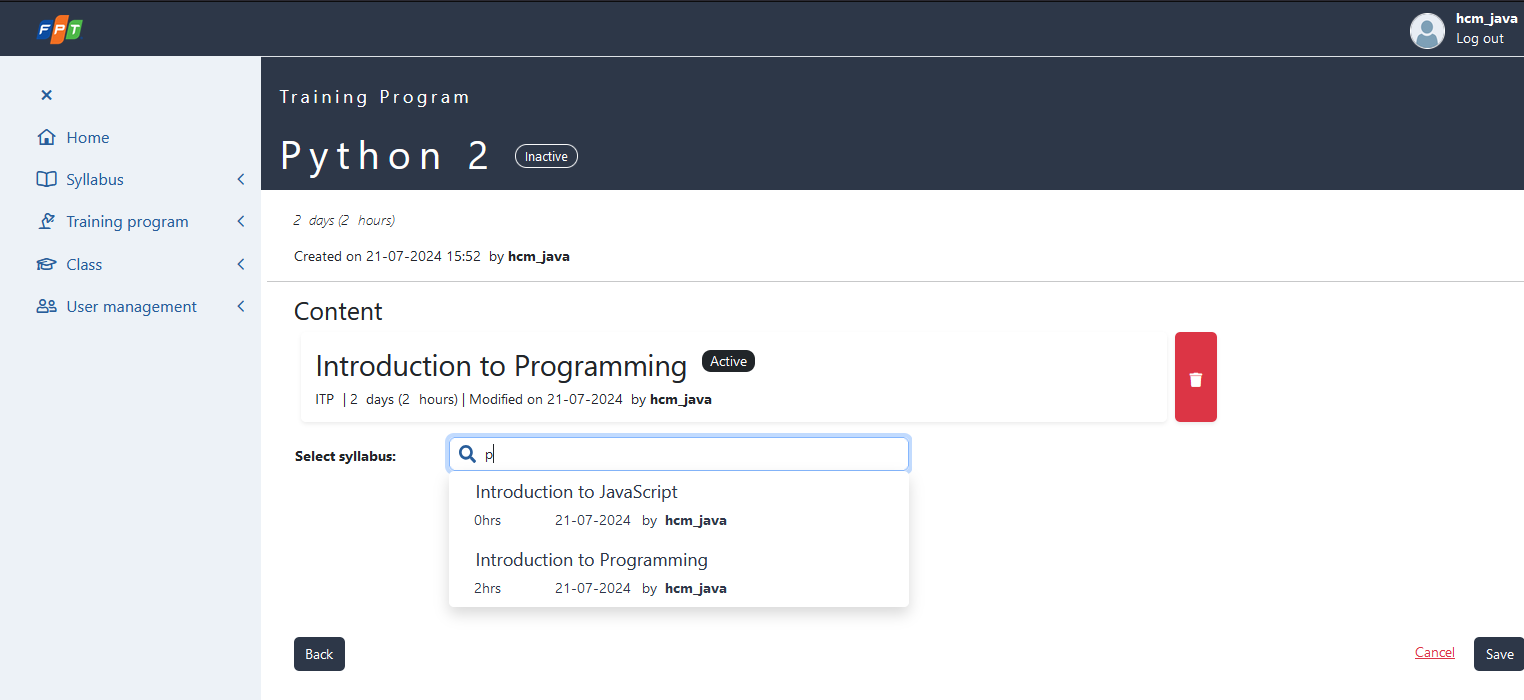
\includegraphics[width=380px]{../meta/ui.program-create-2.png}
\caption[Màn hình tạo mới CTDT]{Màn hình tạo mới CTDT, người dùng nhập thông tin và chọn NDDT thích hợp}
\par
}
\end{figure}
\FloatBarrier

\subsection{Lớp học}

Giao diện chức năng cho phép xem thông tin, xóa, sửa, phân trang, lọc/tìm kiếm các lớp đào tạo.

\begin{figure}[!htb]
{\centering
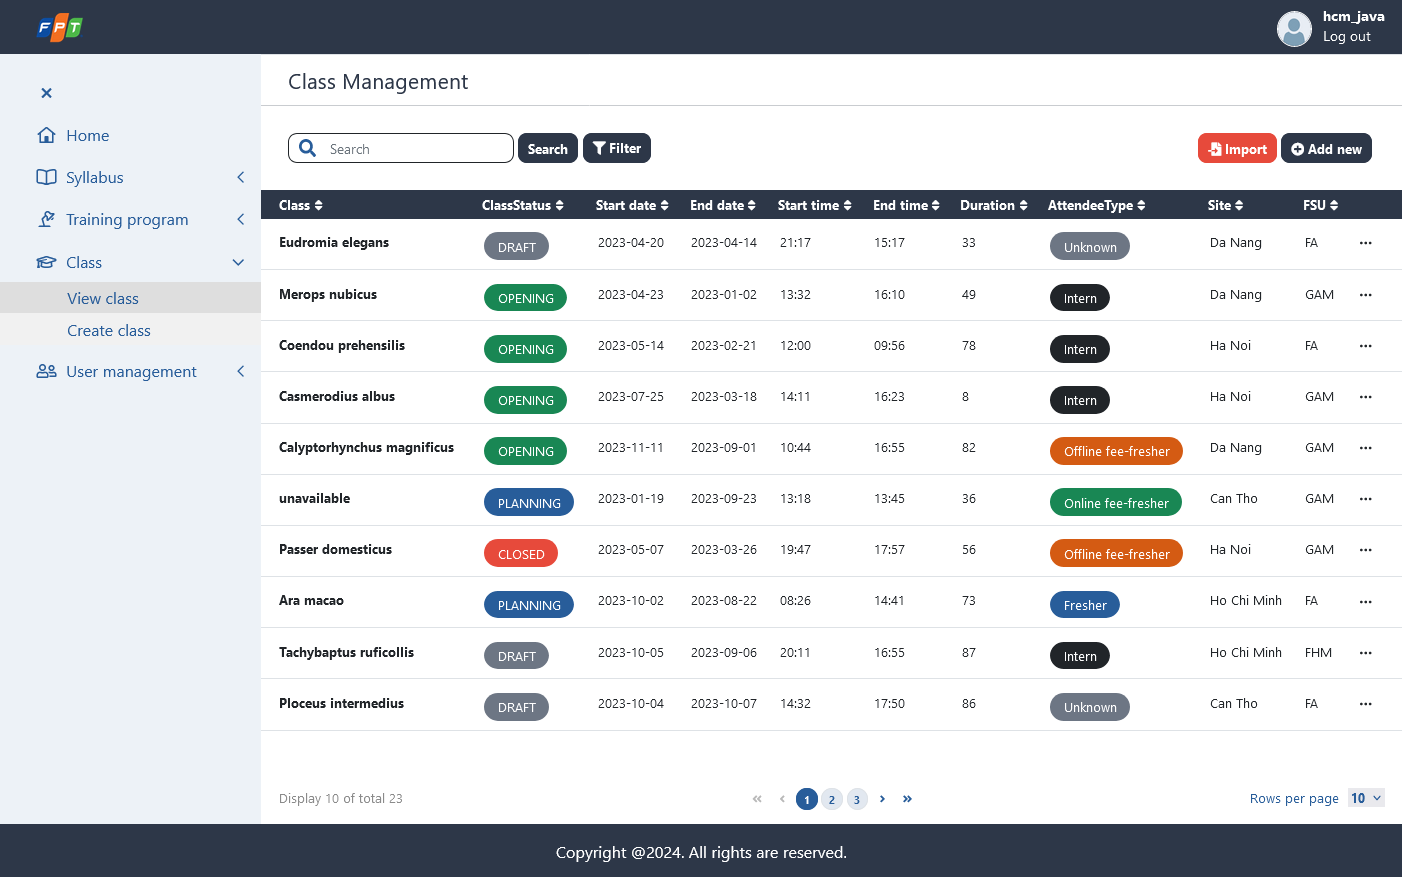
\includegraphics[width=380px]{../meta/ui.class-list.png}
\caption{Màn hình danh sách lớp}
\par
}
\end{figure}
\FloatBarrier

\begin{figure}[!htb]
{\centering
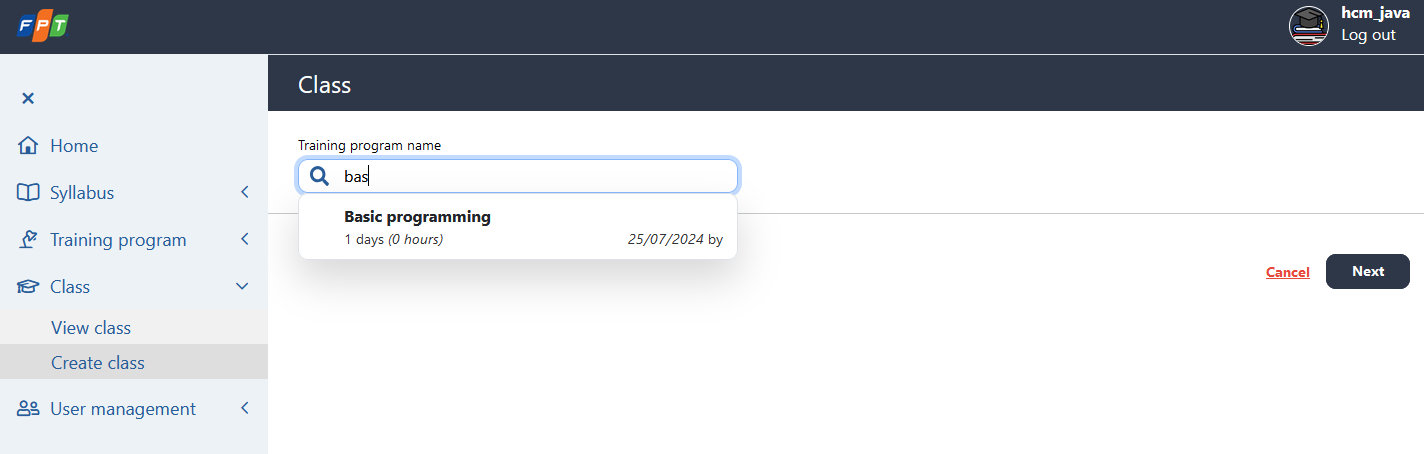
\includegraphics[width=380px]{../meta/ui.class-create1.png}
\caption[Màn hình tạo lớp học]{Màn hình tạo lớp học, người dùng chọn CTDT phù hợp}
\par
}
\end{figure}
\FloatBarrier

\begin{figure}[!htb]
{\centering
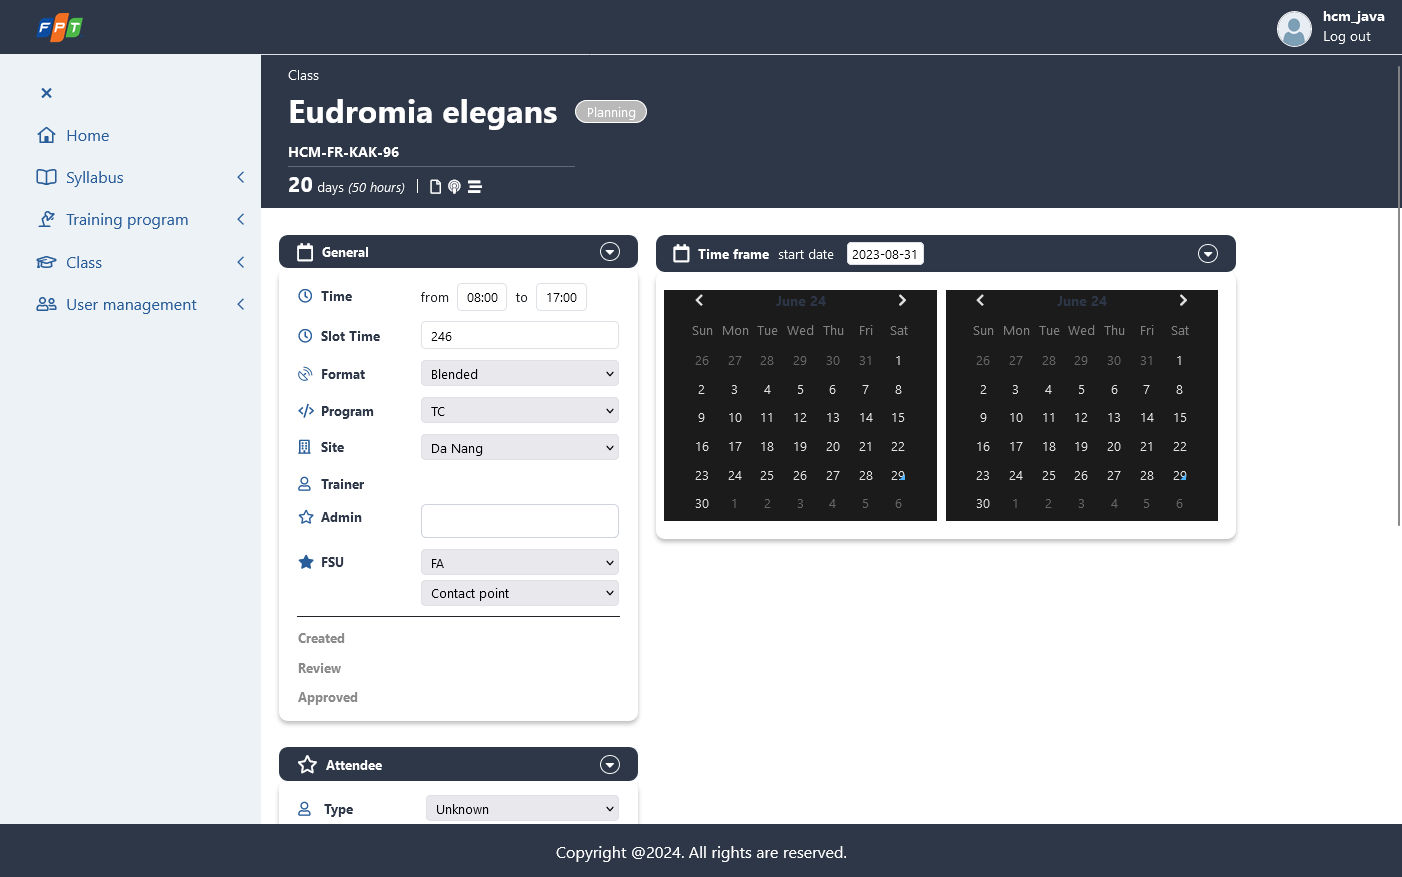
\includegraphics[width=380px]{../meta/ui.class-detail.png}
\caption{Màn hình Thông tin lớp học 1}
\par
}
\end{figure}
\FloatBarrier

\begin{figure}[!htb]
{\centering
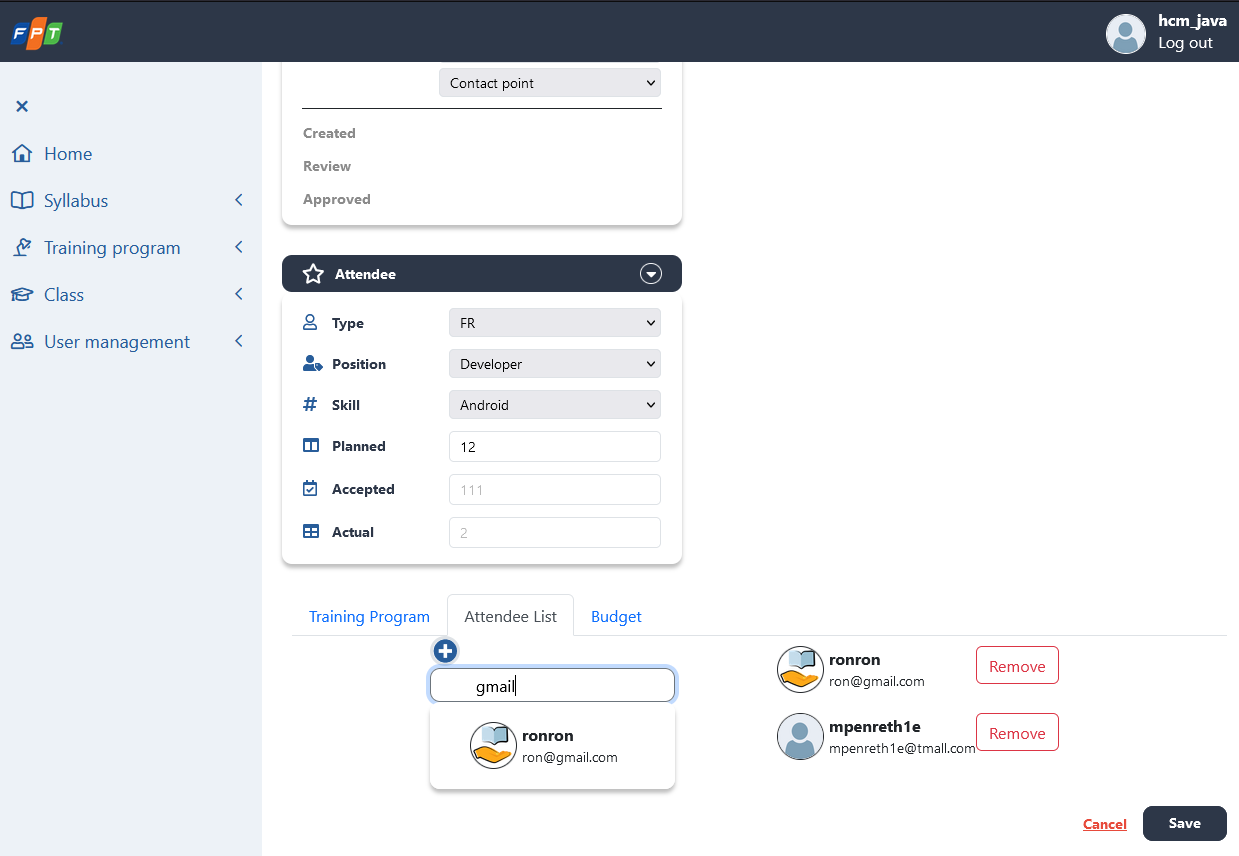
\includegraphics[width=380px]{../meta/ui.class-attendee.png}
\caption{Màn hình thêm học viên vào lớp}
\par
}
\end{figure}
\FloatBarrier

\begin{figure}[!htb]
{\centering
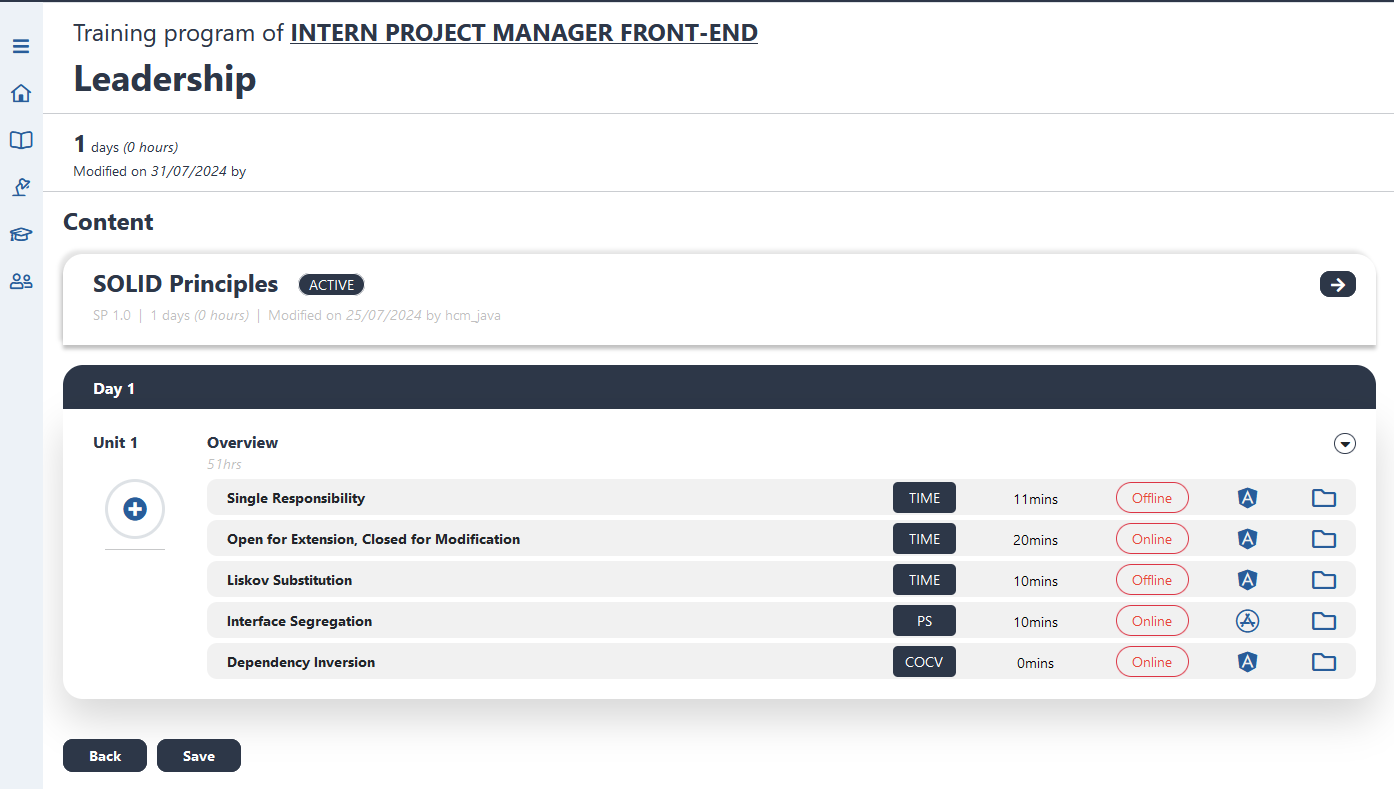
\includegraphics[width=380px]{../meta/ui.class-add-trainer.png}
\caption[Màn hình thêm trainer]{Màn hình thêm trainer vào từng unit bên trong NDDT}
\par
}
\end{figure}
\FloatBarrier

\subsection{Lọc và tìm kiếm}

\begin{figure}[!htb]
{\centering
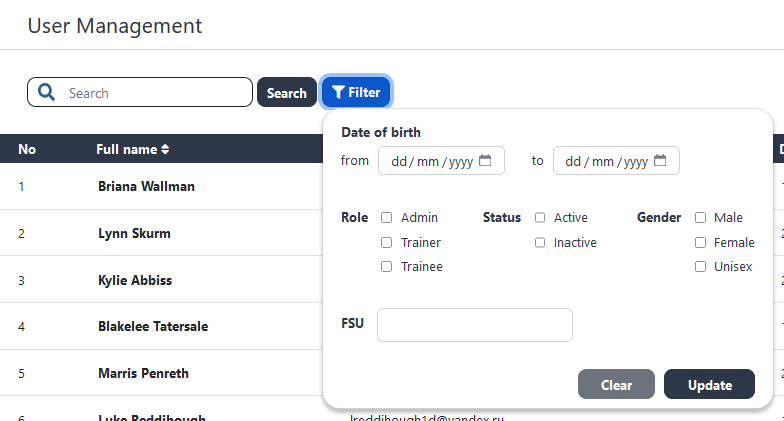
\includegraphics[width=380px]{../meta/ui.user-filter.png}
\caption{Lọc / tìm kiếm user}
\par
}
\end{figure}
\FloatBarrier

\begin{figure}[!htb]
{\centering
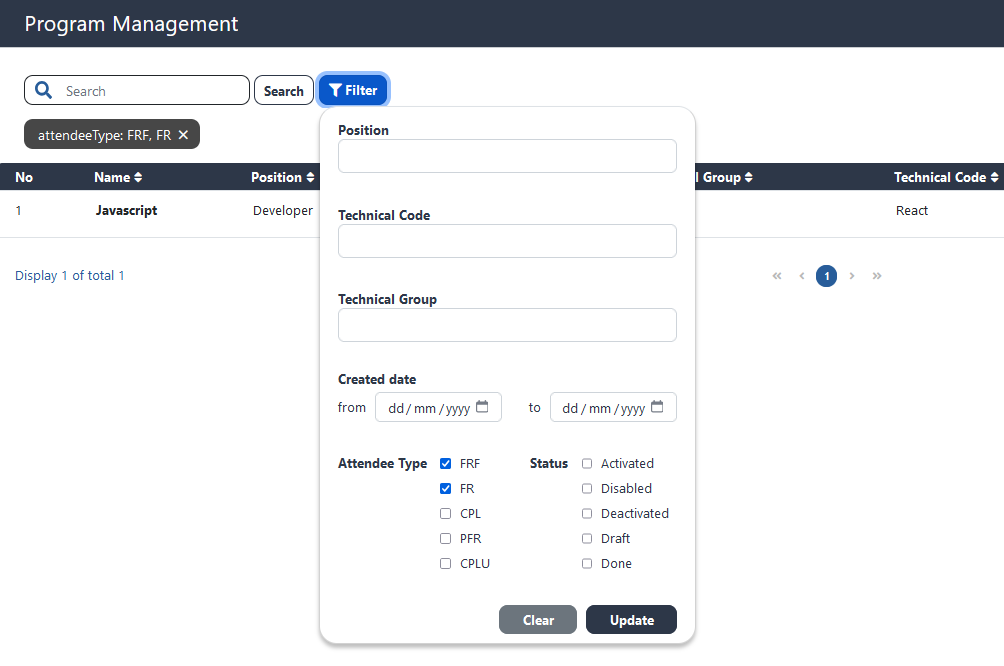
\includegraphics[width=380px]{../meta/ui.program-filter.png}
\caption{Lọc / tìm kiếm CTDT}
\par
}
\end{figure}
\FloatBarrier

\begin{figure}[!htb]
{\centering
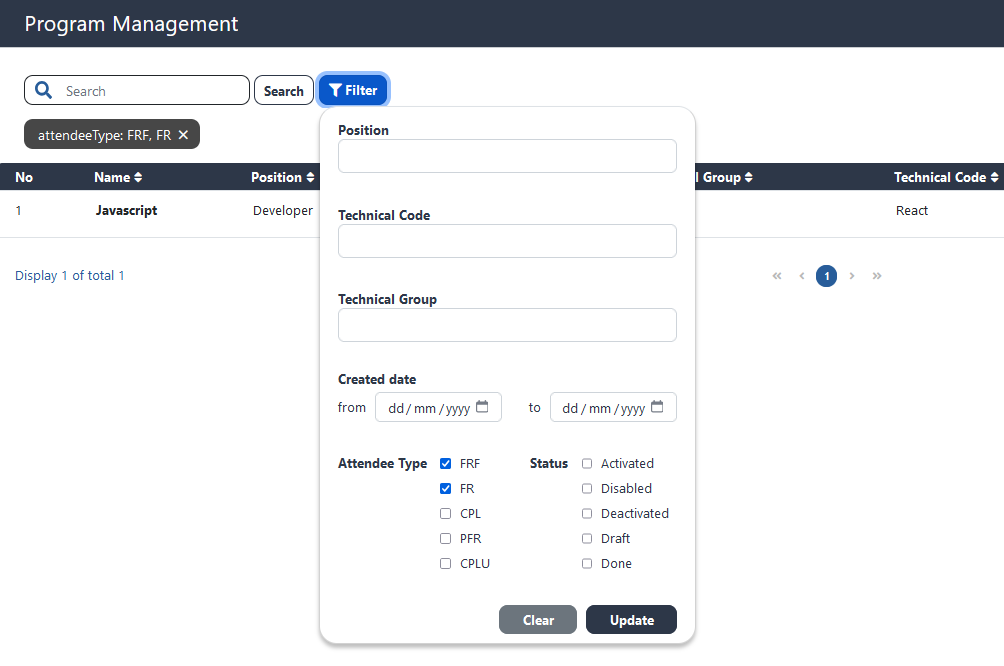
\includegraphics[width=380px]{../meta/ui.program-filter.png}
\caption{Lọc / tìm kiếm lớp đào tạo}
\par
}
\end{figure}
\FloatBarrier

\begin{figure}[!htb]
{\centering
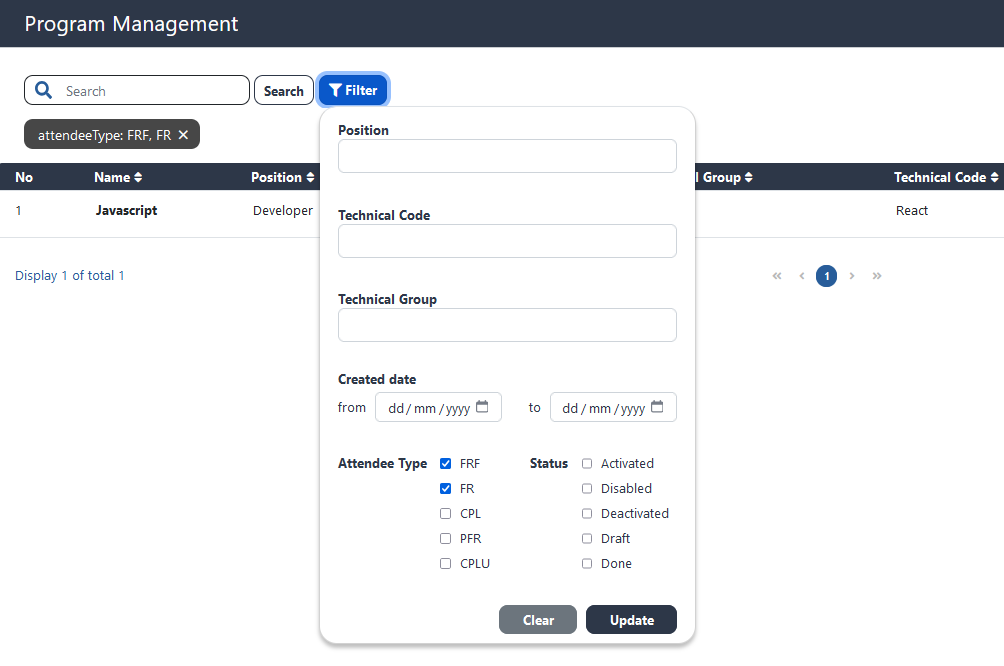
\includegraphics[width=380px]{../meta/ui.program-filter.png}
\caption{Lọc / tìm kiếm người dùng}
\par
}
\end{figure}
\FloatBarrier

\subsection{Import từ file CSV}

Chức năng import data từ file CSV người dùng đã chuẩn bị sẵn, có các tùy chỉnh 
để ghi đè / bỏ qua / cho phép trùng thông tin nếu trường thông tin đã tồn tại.

{\centering
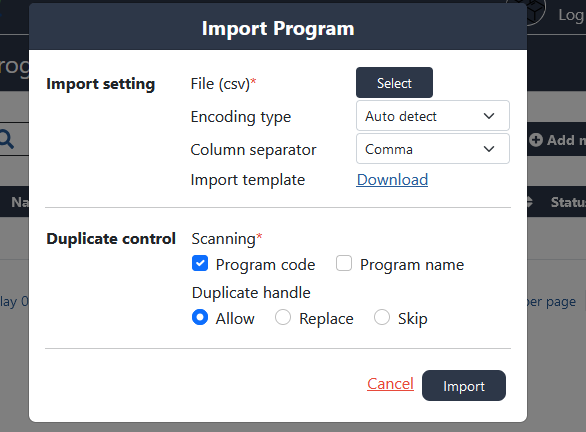
\includegraphics[width=280px]{../meta/ui.program-import.png}
\par
}
{\centering
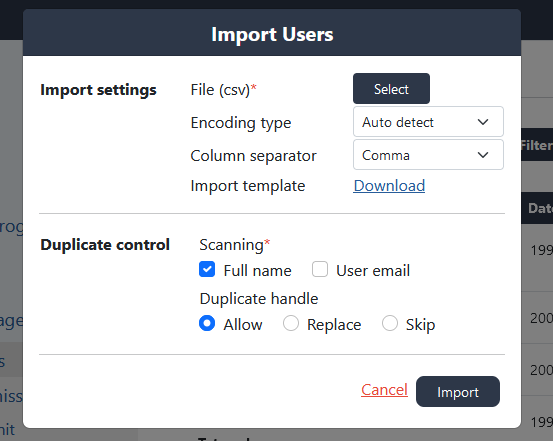
\includegraphics[width=280px]{../meta/ui.user-import.png}
\par
}
{\centering
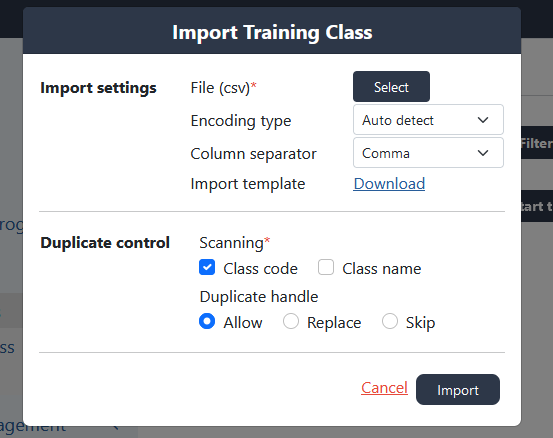
\includegraphics[width=280px]{../meta/ui.class-import.png}
\par
}

\begin{figure}[!htb]
{\centering
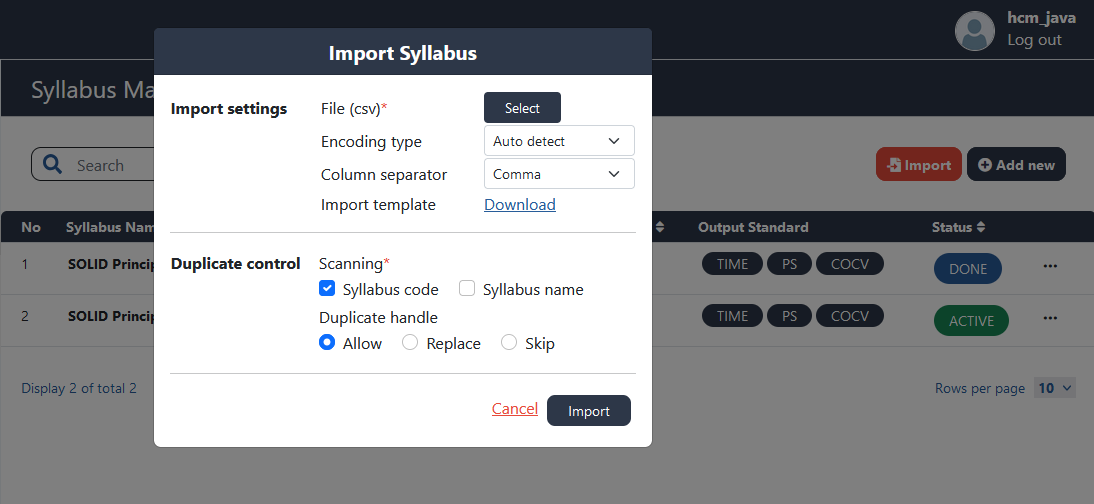
\includegraphics[width=280px]{../meta/ui.syllabus-import.png}
\caption{Import CSV cho NDDT, CTDT, lớp đào tạo, user}
\par
}
\end{figure}
\FloatBarrier

\subsection{Báo cáo lớp học}

\begin{figure}[!htb]
{\centering
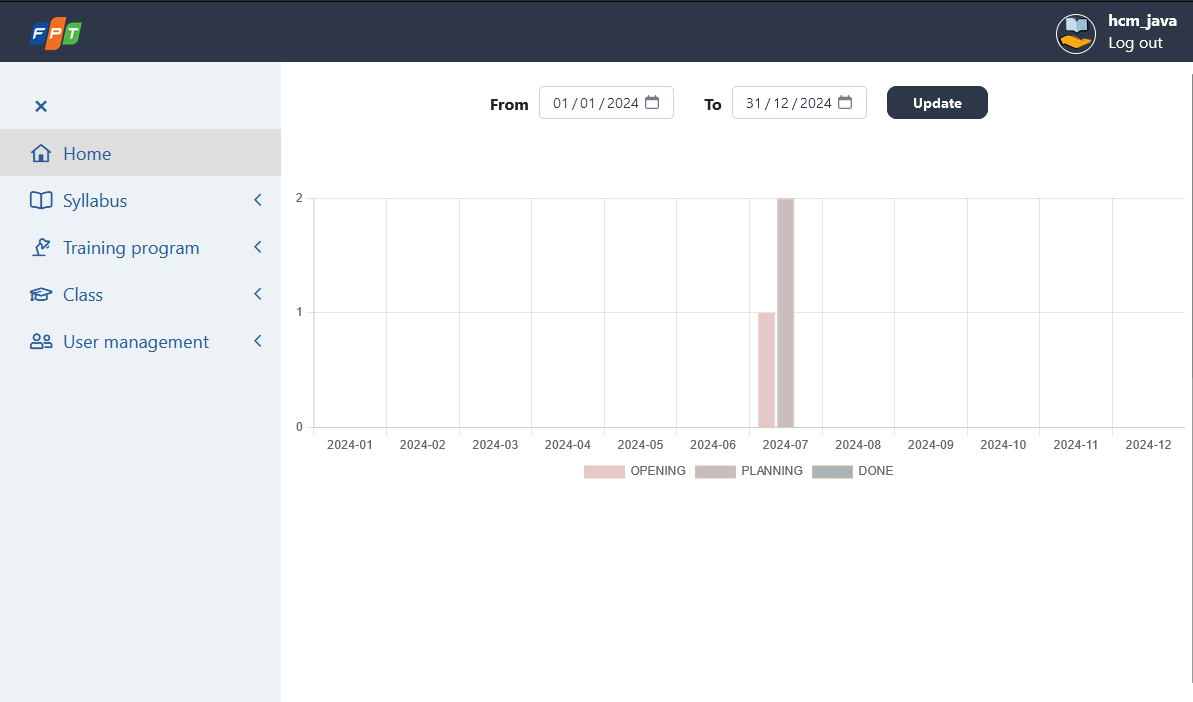
\includegraphics[width=380px]{../meta/ui.class-chart.png}
\caption{Báo cáo lớp học theo tháng}
\par
}
\end{figure}
\FloatBarrier

\subsection{Các thông tin bổ sung}

Các chức năng dưới đây được sử dụng cho việc tạo và quản lý các thông tin bổ trợ,
bao gồm xem, tạo, chỉnh sửa, xóa, tìm kiếm.

\textbf{Phương thức giảng dạy}

{\centering
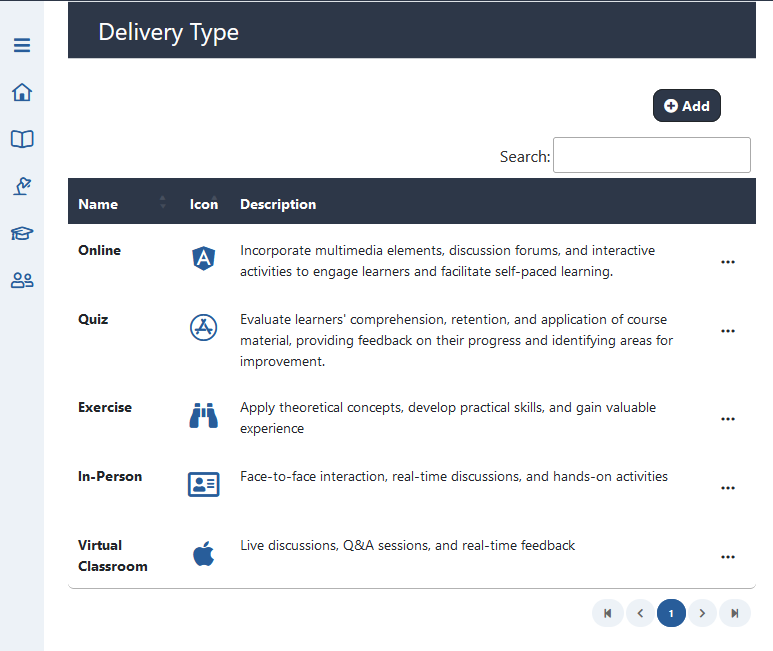
\includegraphics[height=200px]{../meta/ui.deli-list.png}
\par
}

\begin{figure}[!htb]
{\centering
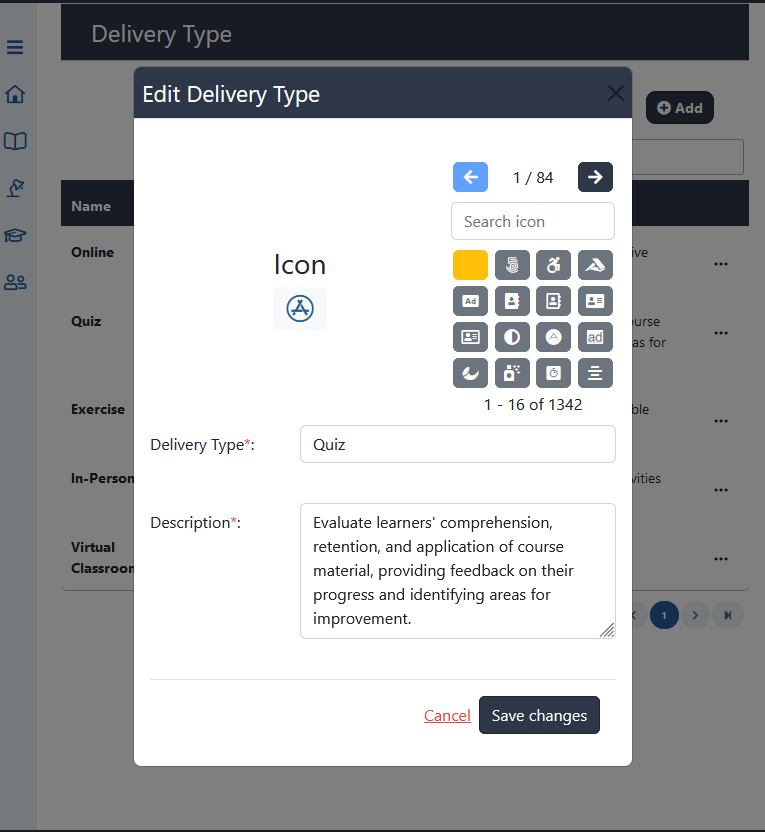
\includegraphics[height=200px]{../meta/ui.deli-create.png}
\caption{Màn hình phương thức giảng dạy}
\par
}
\end{figure}
\FloatBarrier

Giao diện tương tự cho các thông tin về
\textbf{Tiêu chuẩn đầu ra},
\textbf{Đơn vị làm việc},
\textbf{Vị trí},
\textbf{Kỹ năng},
\textbf{Thông tin liên lạc},\dots

\subsection{Quản lý hệ thống}

Các chức năng dưới đây giúp cho đội vận hành, phát triển ứng dụng có thể theo dõi hệ thống, phát hiện và sửa lỗi khi có vấn đề xảy ra.

\begin{figure}[!htb]
{\centering
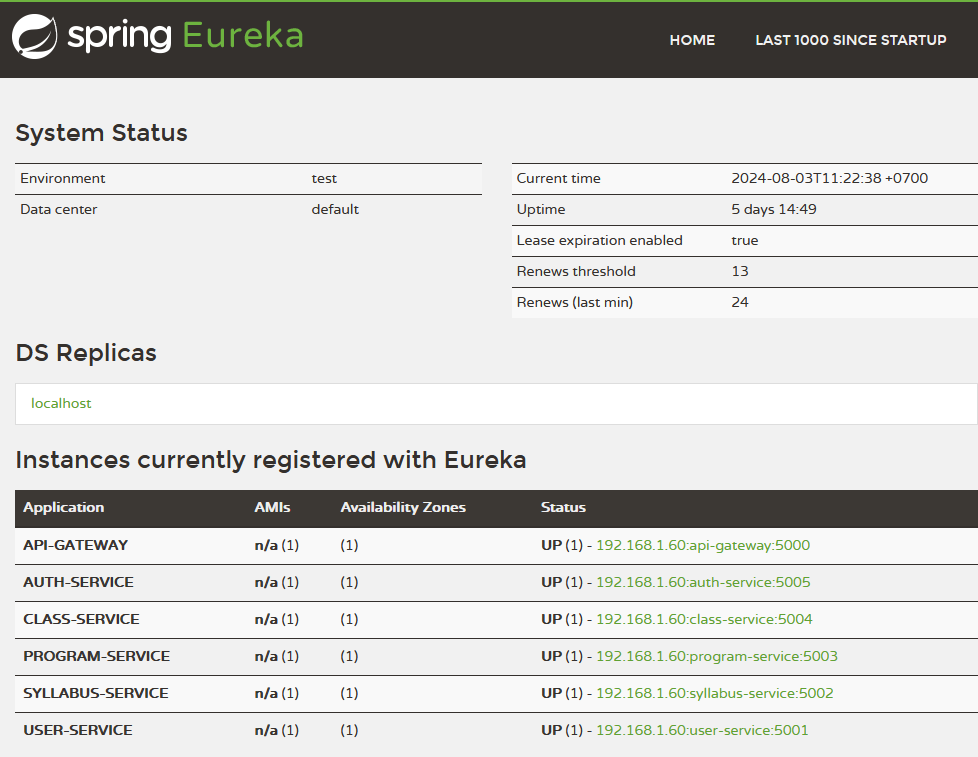
\includegraphics[width=380px]{../meta/ui.eureka.png}
\caption[Màn hình Eureka]{Eureka hiển thị tất cả các service và số instance của service đó}
\par
}
\end{figure}
\FloatBarrier

{\centering
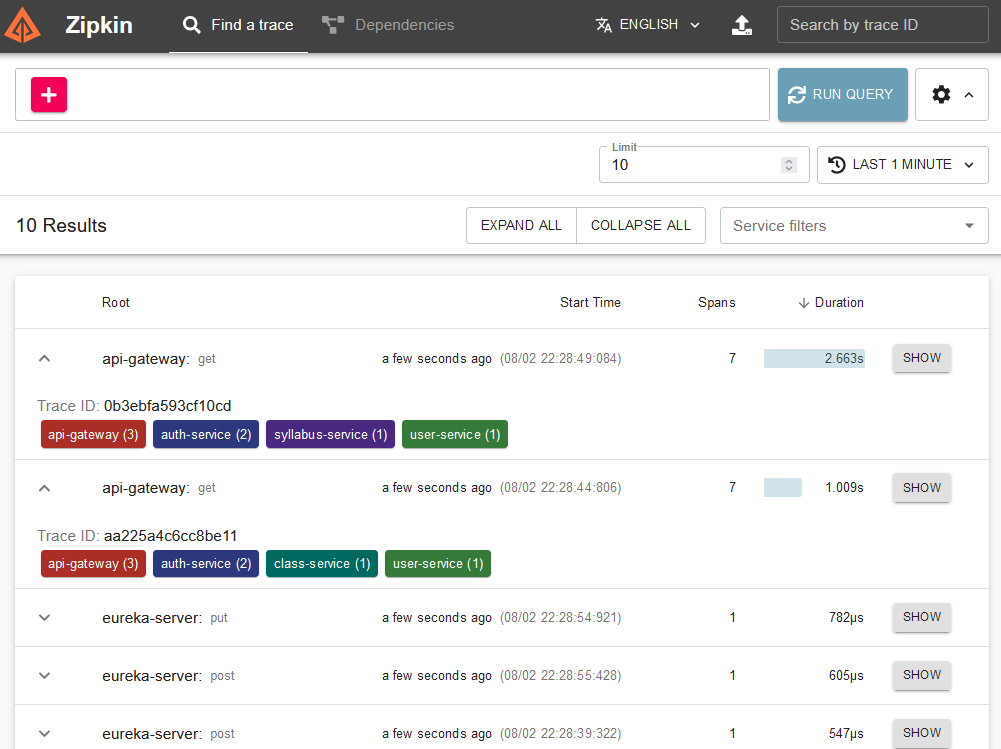
\includegraphics[width=380px]{../meta/ui.zipkin-1.png}
\par
}

\begin{figure}[!htb]
{\centering
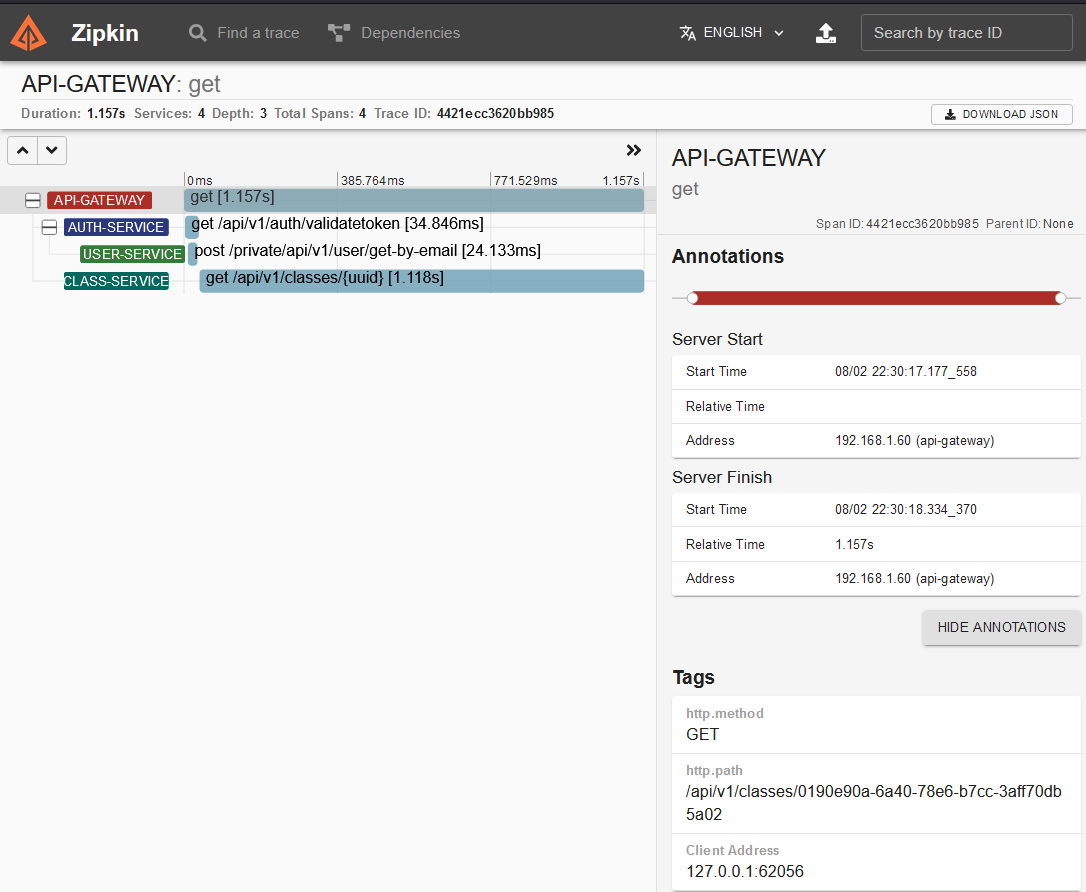
\includegraphics[width=380px]{../meta/ui.zipkin-2.png}
\caption[Màn hình Zipkin]{Zipkin hiển thị đường đi và thời gian của các request đi qua hệ thống}
\par
}
\end{figure}
\FloatBarrier

\begin{figure}[!htb]
{\centering
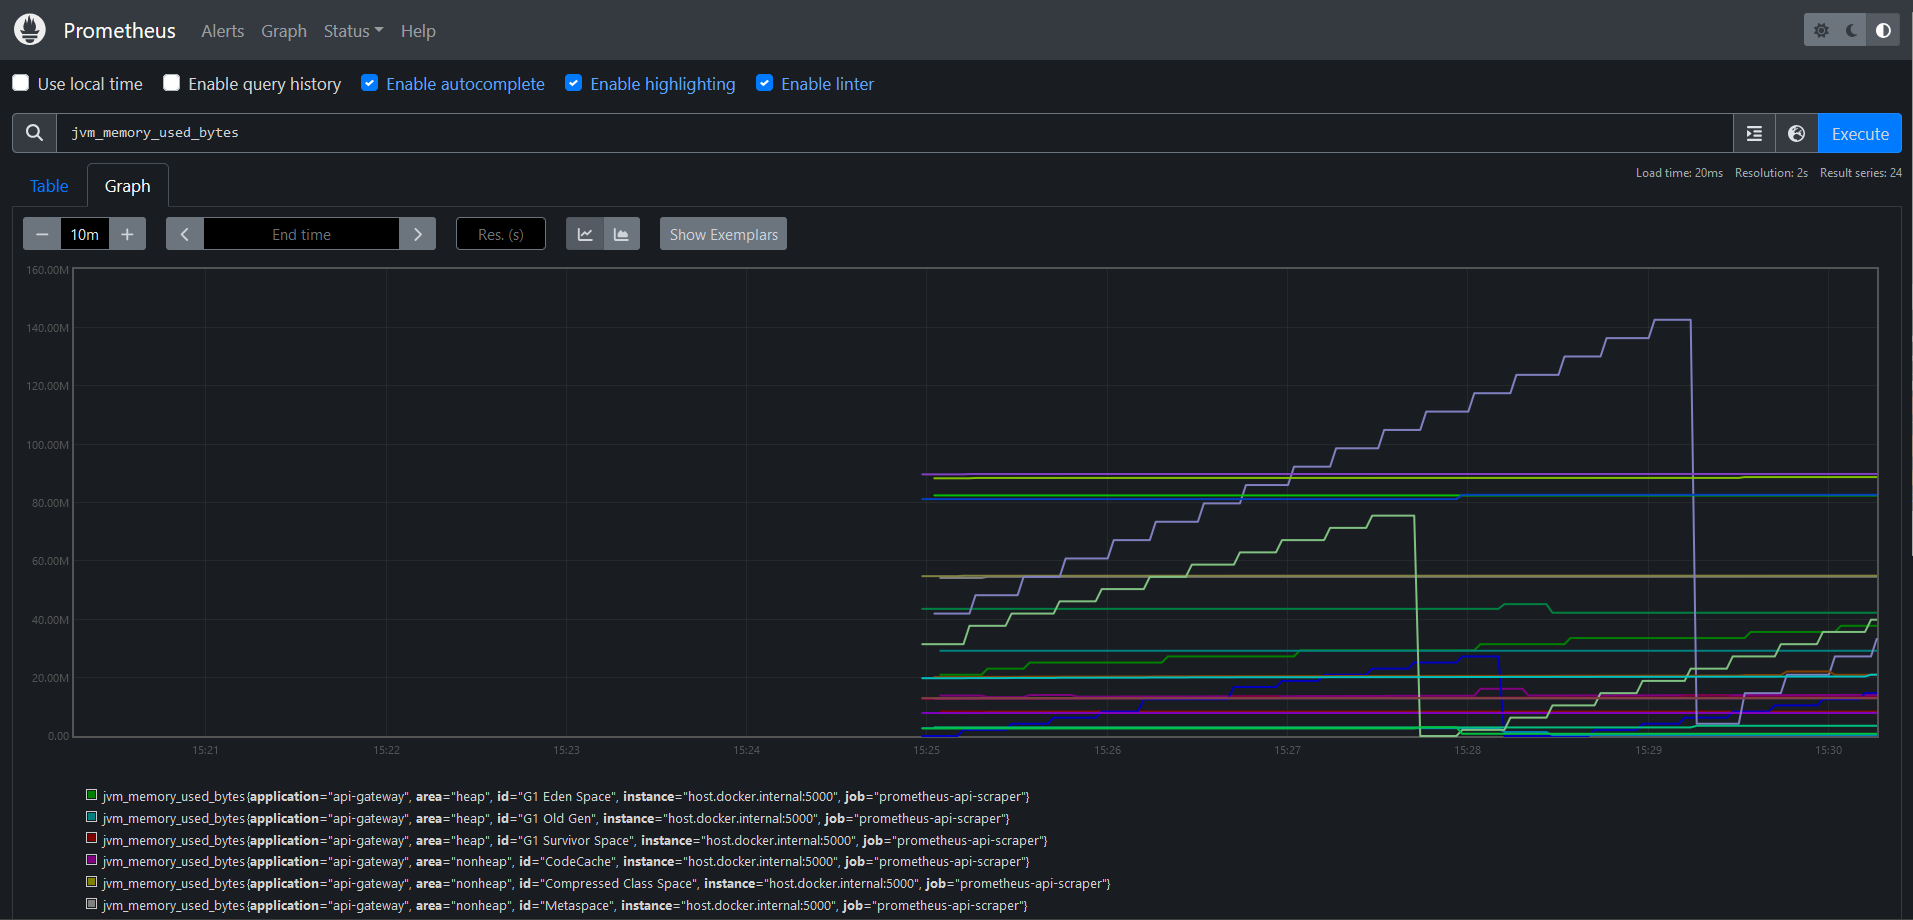
\includegraphics[width=380px]{../meta/ui.prometheus.png}
\caption[Màn hình Prometheus]{Màn hình Prometheus, ở đây hiển thị lược đồ lượng bộ nhớ JVM đang sử dụng}
\par
}
\end{figure}
\FloatBarrier

\begin{figure}[!htb]
{\centering
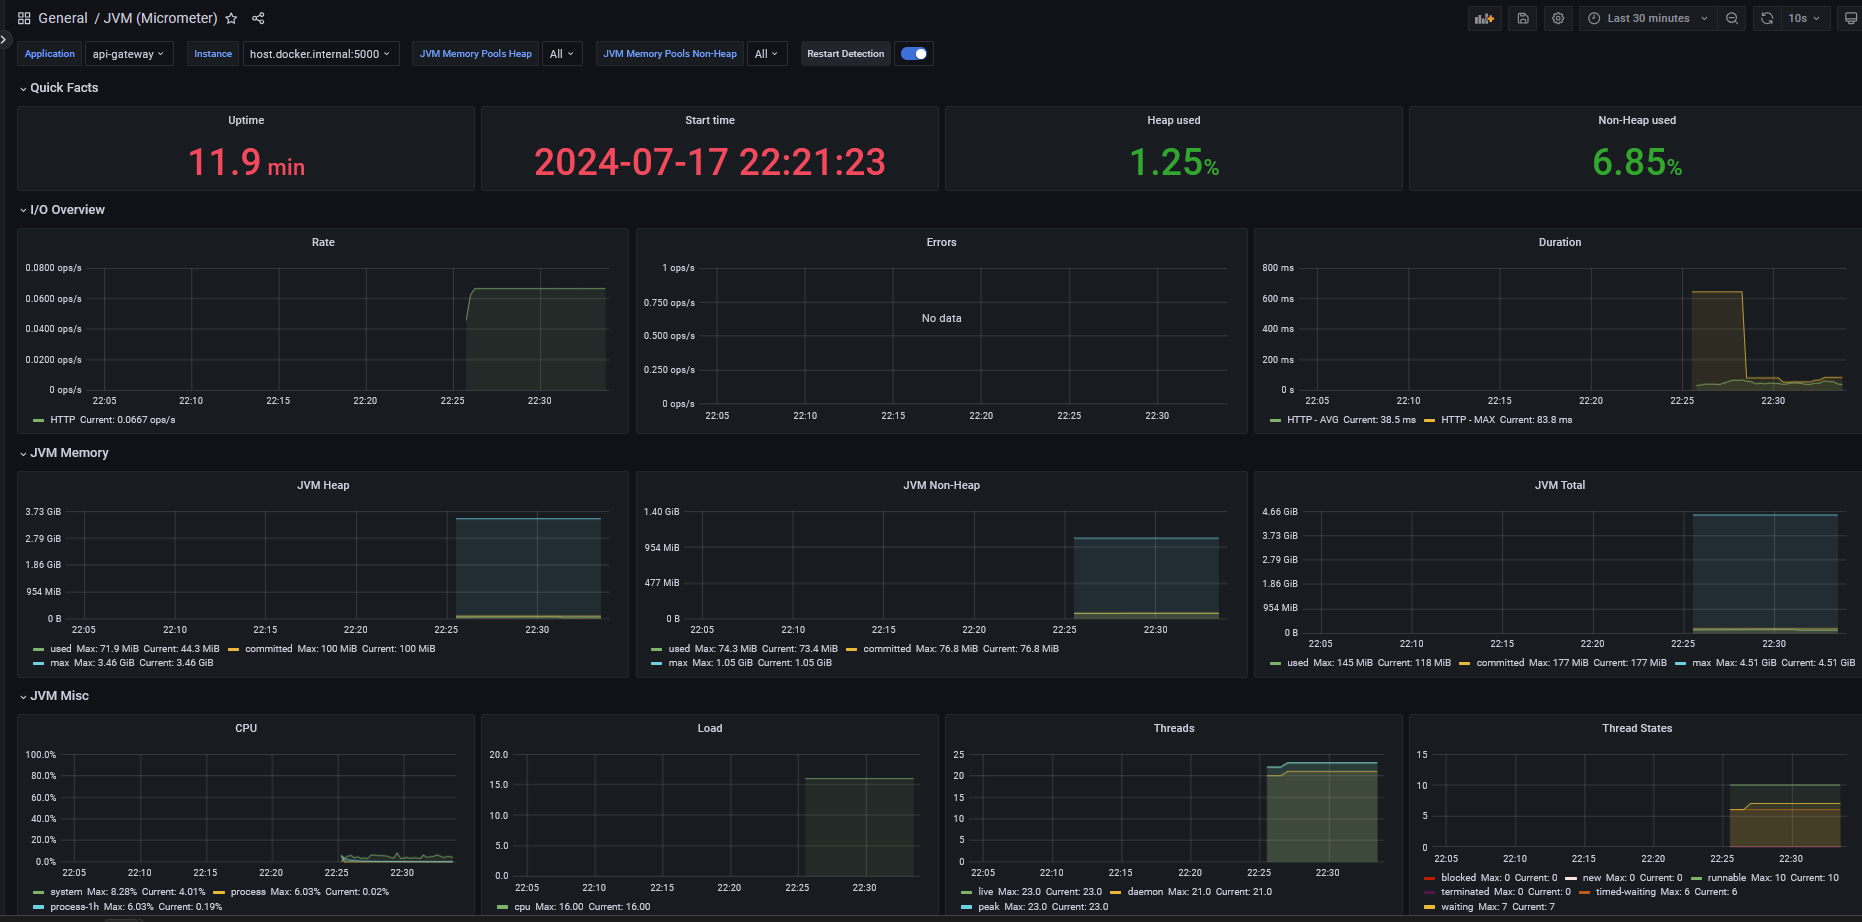
\includegraphics[width=380px]{../meta/ui.grafana.png}
\caption[Grafana dashboard]{Grafana dashboard của service API Gateway, truy xuất dữ liệu từ Prometheus và hiển thị dashboard phục vụ mục đích theo dõi hệ thống.
Các thông tin như thời gian hoạt động, vùng nhớ sử dụng, tải CPU,\dots}
\par
}
\end{figure}
\FloatBarrier

\end{document}

